\documentclass{article}

\usepackage{neurips_2026}
\usepackage[utf8]{inputenc}
\usepackage[T1]{fontenc}
\usepackage{hyperref}
\usepackage{url}
\usepackage{booktabs}
\usepackage{graphicx}
\usepackage{amsmath}
\usepackage{xcolor}
\usepackage{microtype}
\usepackage{tikz}
\usetikzlibrary{arrows.meta}

\graphicspath{{figures/}{auto/}}

% Placeholder macro: any number not yet measured renders red with a dagger.
\newcommand{\ph}[1]{\textcolor{red}{\underline{#1}$^{\dagger}$}}

% Generated result macros; additional protocol and geometry values are documented
% at their source locations. Macro resolution alone does not verify every claim.
% AUTO-GENERATED by autopilot/p8_make_assets.py - do not edit by hand
% Every number in the manuscript resolves through these macros.
\newcommand{\Ntest}{3000}
\newcommand{\Npos}{1466}
\newcommand{\Nneg}{1534}
\newcommand{\Nboot}{10{,}000}
\newcommand{\Nprobes}{23}
\newcommand{\AUCRandomEpFifty}{0.8641}
\newcommand{\CIloRandomEpFifty}{0.8510}
\newcommand{\CIhiRandomEpFifty}{0.8769}
\newcommand{\AUCOracleEpFifty}{0.8740}
\newcommand{\CIloOracleEpFifty}{0.8615}
\newcommand{\CIhiOracleEpFifty}{0.8862}
\newcommand{\AUCEnvelopeEpFifty}{0.8761}
\newcommand{\CIloEnvelopeEpFifty}{0.8635}
\newcommand{\CIhiEnvelopeEpFifty}{0.8879}
\newcommand{\DOracleRandomEpFifty}{+0.0099}
\newcommand{\DOracleRandomEpFiftyCI}{[+0.0051,\,+0.0149]}
\newcommand{\DOracleRandomEpFiftyP}{$<$0.0001}
\newcommand{\DOracleRandomEpFiftyQ}{0.0001}
\newcommand{\DEnvelopeRandomEpFifty}{+0.0120}
\newcommand{\DEnvelopeRandomEpFiftyCI}{[+0.0068,\,+0.0173]}
\newcommand{\DEnvelopeRandomEpFiftyP}{$<$0.0001}
\newcommand{\DEnvelopeRandomEpFiftyQ}{$<$0.0001}
\newcommand{\DOracleEnvelopeEpFifty}{-0.0020}
\newcommand{\DOracleEnvelopeEpFiftyCI}{[-0.0069,\,+0.0029]}
\newcommand{\DOracleEnvelopeEpFiftyP}{0.4114}
\newcommand{\DOracleEnvelopeEpFiftyQ}{0.4114}
\newcommand{\AUCRandomEpSeventyFive}{0.8723}
\newcommand{\CIloRandomEpSeventyFive}{0.8593}
\newcommand{\CIhiRandomEpSeventyFive}{0.8849}
\newcommand{\AUCOracleEpSeventyFive}{0.8836}
\newcommand{\CIloOracleEpSeventyFive}{0.8714}
\newcommand{\CIhiOracleEpSeventyFive}{0.8955}
\newcommand{\AUCEnvelopeEpSeventyFive}{0.8803}
\newcommand{\CIloEnvelopeEpSeventyFive}{0.8677}
\newcommand{\CIhiEnvelopeEpSeventyFive}{0.8922}
\newcommand{\DOracleRandomEpSeventyFive}{+0.0113}
\newcommand{\DOracleRandomEpSeventyFiveCI}{[+0.0063,\,+0.0164]}
\newcommand{\DOracleRandomEpSeventyFiveP}{$<$0.0001}
\newcommand{\DOracleRandomEpSeventyFiveQ}{$<$0.0001}
\newcommand{\DEnvelopeRandomEpSeventyFive}{+0.0080}
\newcommand{\DEnvelopeRandomEpSeventyFiveCI}{[+0.0028,\,+0.0132]}
\newcommand{\DEnvelopeRandomEpSeventyFiveP}{0.0025}
\newcommand{\DEnvelopeRandomEpSeventyFiveQ}{0.0045}
\newcommand{\DOracleEnvelopeEpSeventyFive}{+0.0033}
\newcommand{\DOracleEnvelopeEpSeventyFiveCI}{[-0.0013,\,+0.0079]}
\newcommand{\DOracleEnvelopeEpSeventyFiveP}{0.1491}
\newcommand{\DOracleEnvelopeEpSeventyFiveQ}{0.1677}
\newcommand{\AUCRandomEpHundred}{0.8746}
\newcommand{\CIloRandomEpHundred}{0.8618}
\newcommand{\CIhiRandomEpHundred}{0.8869}
\newcommand{\AUCOracleEpHundred}{0.8855}
\newcommand{\CIloOracleEpHundred}{0.8735}
\newcommand{\CIhiOracleEpHundred}{0.8971}
\newcommand{\AUCEnvelopeEpHundred}{0.8807}
\newcommand{\CIloEnvelopeEpHundred}{0.8683}
\newcommand{\CIhiEnvelopeEpHundred}{0.8926}
\newcommand{\DOracleRandomEpHundred}{+0.0109}
\newcommand{\DOracleRandomEpHundredCI}{[+0.0057,\,+0.0160]}
\newcommand{\DOracleRandomEpHundredP}{$<$0.0001}
\newcommand{\DOracleRandomEpHundredQ}{$<$0.0001}
\newcommand{\DEnvelopeRandomEpHundred}{+0.0062}
\newcommand{\DEnvelopeRandomEpHundredCI}{[+0.0010,\,+0.0113]}
\newcommand{\DEnvelopeRandomEpHundredP}{0.0199}
\newcommand{\DEnvelopeRandomEpHundredQ}{0.0299}
\newcommand{\DOracleEnvelopeEpHundred}{+0.0047}
\newcommand{\DOracleEnvelopeEpHundredCI}{[+0.0004,\,+0.0091]}
\newcommand{\DOracleEnvelopeEpHundredP}{0.0294}
\newcommand{\DOracleEnvelopeEpHundredQ}{0.0378}
\newcommand{\AUCAnatomyTwoEpFifty}{0.8654}
\newcommand{\DAnatomyTwoRandomEpFifty}{+0.0013}
\newcommand{\DAnatomyTwoRandomEpFiftyCI}{[-0.0054,\,+0.0082]}
\newcommand{\DAnatomyTwoRandomEpFiftyP}{0.7101}
\newcommand{\AUCCoverEpFifty}{0.8643}
\newcommand{\DCoverRandomEpFifty}{+0.0002}
\newcommand{\DCoverRandomEpFiftyCI}{[-0.0049,\,+0.0053]}
\newcommand{\DCoverRandomEpFiftyP}{0.9440}
\newcommand{\AUCAncestor}{0.8487}
\newcommand{\NBlack}{431}
\newcommand{\NWhite}{2318}
\newcommand{\NAsian}{251}
\newcommand{\NprobesRace}{19}
\newcommand{\WorstRaceCount}{19}
\newcommand{\BlackAUCOracle}{0.8472}
\newcommand{\BlackCIOracle}{[0.8100,\,0.8804]}
\newcommand{\WhiteAUCOracle}{0.8853}
\newcommand{\RaceGapOracle}{0.0382}
\newcommand{\GapRho}{+0.511}
\newcommand{\GapRhoP}{0.0255}
\newcommand{\SexGapRho}{-0.714}
\newcommand{\SexGapRhoP}{0.0006}
\newcommand{\NprobesSub}{19}
\newcommand{\SubGenderRho}{-0.714}
\newcommand{\SubGenderRhoP}{0.0006}
\newcommand{\SubGenderQ}{0.0042}
\newcommand{\SubGenderBranchRho}{-0.857}
\newcommand{\SubGenderBranchP}{0.0137}
\newcommand{\SubGenderGapMin}{0.0272}
\newcommand{\SubGenderGapMax}{0.0396}
\newcommand{\SubGenderWorst}{female}
\newcommand{\SubGenderWorstN}{19}
\newcommand{\SubRaceRho}{+0.511}
\newcommand{\SubRaceRhoP}{0.0255}
\newcommand{\SubRaceQ}{0.0595}
\newcommand{\SubRaceBranchRho}{+0.429}
\newcommand{\SubRaceBranchP}{0.3374}
\newcommand{\SubRaceGapMin}{0.0475}
\newcommand{\SubRaceGapMax}{0.0935}
\newcommand{\SubRaceWorst}{black}
\newcommand{\SubRaceWorstN}{19}
\newcommand{\SubEthnicityRho}{+0.351}
\newcommand{\SubEthnicityRhoP}{0.1408}
\newcommand{\SubEthnicityQ}{0.1971}
\newcommand{\SubEthnicityBranchRho}{+0.464}
\newcommand{\SubEthnicityBranchP}{0.2939}
\newcommand{\SubEthnicityGapMin}{0.0223}
\newcommand{\SubEthnicityGapMax}{0.0661}
\newcommand{\SubEthnicityWorst}{hispanic}
\newcommand{\SubEthnicityWorstN}{19}
\newcommand{\SubLanguageRho}{+0.275}
\newcommand{\SubLanguageRhoP}{0.2537}
\newcommand{\SubLanguageQ}{0.2537}
\newcommand{\SubLanguageBranchRho}{+0.786}
\newcommand{\SubLanguageBranchP}{0.0362}
\newcommand{\SubLanguageGapMin}{0.0518}
\newcommand{\SubLanguageGapMax}{0.0805}
\newcommand{\SubLanguageWorst}{other languages}
\newcommand{\SubLanguageWorstN}{15}
\newcommand{\SubMaritalRho}{-0.444}
\newcommand{\SubMaritalRhoP}{0.0570}
\newcommand{\SubMaritalQ}{0.0997}
\newcommand{\SubMaritalBranchRho}{-0.714}
\newcommand{\SubMaritalBranchP}{0.0713}
\newcommand{\SubMaritalGapMin}{0.0364}
\newcommand{\SubMaritalGapMax}{0.0654}
\newcommand{\SubMaritalWorst}{single}
\newcommand{\SubMaritalWorstN}{19}
\newcommand{\SubAgeRho}{+0.304}
\newcommand{\SubAgeRhoP}{0.2065}
\newcommand{\SubAgeQ}{0.2409}
\newcommand{\SubAgeBranchRho}{+0.357}
\newcommand{\SubAgeBranchP}{0.4316}
\newcommand{\SubAgeGapMin}{0.0487}
\newcommand{\SubAgeGapMax}{0.0704}
\newcommand{\SubAgeWorst}{$<$60}
\newcommand{\SubAgeWorstN}{18}
\newcommand{\SubSeverityRho}{-0.521}
\newcommand{\SubSeverityRhoP}{0.0222}
\newcommand{\SubSeverityQ}{0.0595}
\newcommand{\SubSeverityBranchRho}{-0.857}
\newcommand{\SubSeverityBranchP}{0.0137}
\newcommand{\SubSeverityGapMin}{0.1286}
\newcommand{\SubSeverityGapMax}{0.1400}
\newcommand{\SubSeverityWorst}{mild ($-6$,$-2$]}
\newcommand{\SubSeverityWorstN}{19}
\newcommand{\NbranchesSub}{7}
\newcommand{\SeverityGapSpread}{0.0114}
\newcommand{\SubAUCMin}{0.8483}
\newcommand{\SubAUCMax}{0.8855}
\newcommand{\SevRandomMild}{0.8164}
\newcommand{\SevRandomModerate}{0.9030}
\newcommand{\SevRandomSevere}{0.9525}
\newcommand{\SevOracleMild}{0.8301}
\newcommand{\SevOracleModerate}{0.9131}
\newcommand{\SevOracleSevere}{0.9588}
\newcommand{\SevEnvelopeMild}{0.8232}
\newcommand{\SevEnvelopeModerate}{0.9103}
\newcommand{\SevEnvelopeSevere}{0.9559}
\newcommand{\SevDeltaMild}{+0.0137}
\newcommand{\SevDeltaModerate}{+0.0102}
\newcommand{\SevDeltaSevere}{+0.0063}
\newcommand{\SevGapRandom}{0.1361}
\newcommand{\SevGapOracle}{0.1286}
\newcommand{\RaceRandomWhite}{0.8741}
\newcommand{\RaceRandomBlack}{0.8325}
\newcommand{\RaceRandomAsian}{0.9033}
\newcommand{\RaceOracleWhite}{0.8853}
\newcommand{\RaceOracleBlack}{0.8472}
\newcommand{\RaceOracleAsian}{0.9189}
\newcommand{\BlackGainOracle}{+0.0147}
\newcommand{\FTOracleMeanpool}{0.8947}
\newcommand{\FTRandomMeanpool}{0.8868}
\newcommand{\FTDelta}{+0.0079}
\newcommand{\FTOracleBest}{0.8947}
\newcommand{\FTRandomBest}{0.8878}
\newcommand{\FTDeltaBest}{+0.0069}

% Generated by autopilot/make_delivered_assets.py; do not edit values.
\newcommand{\DTFullImages}{576}
\newcommand{\DTValidGuides}{573}
\newcommand{\DTTissueTruncation}{300}
\newcommand{\DTZeroContext}{55}
\newcommand{\DTLegacyFloorMiss}{358}
\newcommand{\DTLegacyTruncation}{300}
\newcommand{\DTLegacyZeroContext}{55}
\newcommand{\DTLegacyScoredMass}{78.51}
\newcommand{\DTLegacyDeliveredMass}{74.57}
\newcommand{\DTLegacyContextMean}{10.13}
\newcommand{\DTPrefixFloorMiss}{320}
\newcommand{\DTPrefixTruncation}{0}
\newcommand{\DTPrefixZeroContext}{38}
\newcommand{\DTPrefixScoredMass}{78.56}
\newcommand{\DTPrefixDeliveredMass}{78.56}
\newcommand{\DTPrefixContextMean}{11.24}
\newcommand{\DTGuardFloorMiss}{0}
\newcommand{\DTGuardTruncation}{0}
\newcommand{\DTGuardZeroContext}{1}
\newcommand{\DTGuardScoredMass}{78.56}
\newcommand{\DTGuardDeliveredMass}{78.56}
\newcommand{\DTGuardContextMean}{15.12}
\newcommand{\DTGPUObservations}{2}
\newcommand{\DTGPUCases}{3}
\newcommand{\DTGPUGuardChanges}{0}


% ARM DISPLAY NAMES. Defined once so a rename is a one-line change and cannot
% drift between prose, tables and figure captions. \ArmBest is the strongest
% arm: it locates a retinal band by a per-column intensity centroid and uses NO
% segmentation model and NO ground-truth labels. Named for what it computes.
\newcommand{\ArmBest}{\textsc{centroid}}

\title{Anatomy-Guided Masking for I-JEPA\\
Representation Learning on Retinal OCT}

\author{}

\begin{document}

\maketitle

\begin{abstract}
Anatomy-guided masking is motivated by concentrating representation learning
on informative tissue, but prediction also requires useful visible context.
We study six I-JEPA masking-policy implementations on volumetric retinal OCT,
using a 2D B-scan encoder and a frozen volume-level linear probe for glaucoma
classification (FairVision, $N{=}\Ntest$). The encoders descend from a shared
checkpoint, with one continuation per policy. Segmenter-guided rectangular
target placement improves AUC over uniform placement by
$\DEnvelopeRandomEpFifty$ at epoch 50. A segmentation-free intensity-centroid
policy improves it by $\DOracleRandomEpHundred$ at epoch 100.
Both policies have positive paired differences from uniform placement at all
three evaluated epochs. Their difference is unresolved at epochs 50 and 75;
the centroid policy is higher at epoch 100, which does not establish
equivalence between the methods. Greater tissue purity or coverage is not
consistently beneficial across the other implementations: an early,
incompletely documented anatomy-shaped continuation has higher AUC than its
rectangle comparator, whereas later shaped and
coverage-constrained policies do not consistently improve the uniform baseline.
Auditing delivered masks reveals changes in visible context, target area and
loss weighting, including target truncation after coverage-based placement.
These comparisons therefore do not isolate the effect of anatomical coverage.
Background-feature diagnostics further motivate distinguishing target content
from information retained in context, without establishing a causal mechanism.
The results support tissue-directed placement in these runs, not a ranking
over retrainings: the test split was repeatedly inspected, and subgroup and
low-label analyses remain exploratory.
\end{abstract}

\section{Introduction}

Self-supervised learning has become the default route to representation quality
in medical imaging, where expert annotation is expensive and pathology is
rare~\citep{azizi2021big,zhou2023retfound,qiu2024visionfm}. Joint-embedding
predictive architectures such as I-JEPA~\citep{assran2023ijepa} learn by
predicting the \emph{representation} of masked target blocks from a visible
context block, avoiding pixel reconstruction and its bias toward high-frequency
detail~\citep{he2022mae,xie2022simmim}.

I-JEPA samples its targets geometrically: rectangles placed uniformly at random.
In natural images this is defensible, since informative content is spread
broadly across the frame. In a retinal OCT B-scan it is not obviously so. A
large fraction of the image is dark vitreous and background. The diagnostic
signal for glaucoma is concentrated in a thin band of retinal tissue. This
motivates an intuitive hypothesis, one that several recent methods
adopt~\citep{li2022semmae,li2024anatomask,wang2025maskwhatmatters,shi2022adios}:
\emph{direct the predictive objective at clinically meaningful anatomy rather
than at arbitrary image regions.}

Selecting targets and retaining context are coupled decisions. Hiding more
tissue can increase the amount to predict while removing the evidence needed
to predict it. Random targets can also include background whose latent features
depend on surrounding tissue. We therefore examine anatomy-directed target
selection, encoder-visible context and background supervision jointly, rather
than assume that increasing anatomical coverage must help.

We compare six masking-policy implementations, from uniformly placed rectangles
to tissue-directed rectangles and anatomy-shaped targets. The encoders descend
from a shared pretrained checkpoint, but implementation, collation and historical
continuation details differ. We use matched frozen-probe comparisons where
available and measure the masks delivered to the model, rather than infer them
from configuration names.

The tissue-directed rectangle policies outperform uniform placement in the
observed continuations. The centroid policy uses image intensity rather than
a segmentation model and has the highest epoch-100 point estimate.
The anatomy-shaped results are mixed, including a positive early comparison.
Neither these outcomes nor the coverage-constrained arm isolates how much
anatomy should be hidden: target area, retained context and the number of
supervised target tokens also change. This motivates an implementation audit
before a stronger claim about the masking mechanism.

\paragraph{Contributions.}
\begin{itemize}
\setlength{\itemsep}{0pt}\setlength{\parskip}{0pt}
\item A six-policy study of target selection for OCT representation learning,
      with a shared encoder ancestry and matched frozen-probe comparisons (every probe
      fitted is listed in Appendix~\ref{app:allprobes}).
\item Positive run-level results for segmenter-guided and segmentation-free
      rectangle placement, with mixed outcomes for more anatomically specific
      implementations.
\item An audit of delivered target and context geometry that identifies why
      the tested implementations do not isolate anatomical coverage. Additional
      background, low-label and subgroup analyses delimit the interpretation.
\end{itemize}

\section{Related work}

\paragraph{Masked image modelling and JEPAs.}
Masked autoencoders reconstruct pixels~\citep{he2022mae,xie2022simmim};
BEiT~\citep{bao2022beit} and iBOT~\citep{zhou2022ibot} predict discrete tokens;
data2vec~\citep{baevski2022data2vec} and I-JEPA~\citep{assran2023ijepa} predict
latent representations. Video and 3D extensions follow the same
template~\citep{bardes2024vjepa,chen2023mim3d,taleb20203dssl}. Other JEPA
formulations also change the training objective or prediction structure
rather than only the masking distribution~\citep{balestriero2025lejepa,he2025dseqjepa}.

\paragraph{Region selection and prediction structure.}
DSeq-JEPA~\citep{he2025dseqjepa} combines attention-derived region selection
with sequential prediction from more salient regions to less salient regions.
Its most salient region supplies context rather than being the first prediction
target. In its reported factorial ablation, discriminative selection with a
flat predictor does not improve on uniform I-JEPA in the reported single-run
point estimates, without a significance inference,
whereas their joint sequential design does. The regions, saliency source,
conditioning and datasets differ from ours; this is not a direct test of
retinal anatomy guidance. It demonstrates why successful guided prediction
cannot be reduced to the rule ``hide more important tissue.'' I-JEPA's own
context-scale ablation likewise motivates retaining informative context
alongside sufficiently large prediction targets~\citep{assran2023ijepa}.

\paragraph{Informed masking.}
A substantial line of work argues that \emph{what} is masked matters.
ADIOS~\citep{shi2022adios} learns an adversarial masking model;
SemMAE~\citep{li2022semmae} uses learned semantic parts;
AttMask~\citep{kakogeorgiou2022attmask} masks by attention;
HardPatches~\citep{wang2023hpm} and AutoMAE~\citep{chen2023automae}
target difficulty. In the medical domain, AnatoMask~\citep{li2024anatomask},
AnatomyMAE~\citep{ceballosarroyo2026anatomymae},
MSMAE~\citep{mao2023msmae}, and VasoMIM~\citep{huang2026vasomim} explicitly
steer masking toward anatomy, and \citet{wang2025maskwhatmatters} argue directly
for masking clinically relevant regions. Our study examines that premise
through run-level comparisons and a delivered-task audit on one task.

\paragraph{Evidence that informed masking is not uniformly better.}
The effect depends on the objective and masking construction. Original MAE
uses random patches and reports better performance than its block and grid
alternatives~\citep{he2022mae}. SemMAE's scheduled part-based masking improves
its reported linear-probe result, while masking whole parts throughout training
does not; its part-map ablation also shows sensitivity to the guide
source~\citep{li2022semmae}. Conversely, anatomy-biased masking helps in a
fine-tuned CT aneurysm-detection pipeline that also studies crop selection and
distance-map reconstruction~\citep{ceballosarroyo2026anatomymae}. These are
different tasks and interventions, not evidence for a universal masking rule.
Our OCT comparison asks which conclusions survive a direct audit of target
selection and retained context under latent prediction. Additional contextual
comparisons are recorded in Appendix~\ref{app:counter}.

\paragraph{Retinal foundation models, OCT, and fairness.}
RETFound~\citep{zhou2023retfound}, VisionFM~\citep{qiu2024visionfm},
URFound~\citep{yu2024urfound}, and OCTCube~\citep{liu2026octcube} pretrain on
large retinal corpora. OCT-specific masked modelling is explored by
\citet{pissas2024octmim}. MIRAGE~\citep{morano2025mirage} provides multimodal
OCT segmentation and supplies the anatomical guidance used by several of our
arms, and deep glaucoma detection from OCT is
established~\citep{maetschke2019glaucoma,ran2019glaucoma,noury2022glaucoma}.
Performance disparities across demographic groups are widely
documented~\citep{seyyedkalantari2021underdiagnosis,larrazabal2020gender,gichoya2022race}.
FairVision~\citep{luo2024fairvision} and Harvard-GF~\citep{luo2024harvardgf}
provide OCT data with demographic attributes, and
FairMedFM~\citep{jin2024fairmedfm} and \citet{shi2025equitable} benchmark
fairness for medical foundation models.

\section{Method: anatomy-guided target selection}
\label{sec:policies}

We compare five policy families, represented by six historical implementations,
with a shared encoder ancestry and a common
frozen-probe protocol. The intended intervention is target selection; differences
in delivered geometry and historical continuation are reported separately.

\subsection{Background}

I-JEPA samples from the token grid of an image a context block and $M$ target
blocks, which need not cover it. A context encoder embeds the visible tokens. A predictor maps that
embedding plus positional queries to predicted representations of the target
tokens. An exponential-moving-average target encoder supplies the regression
targets. With a $16{\times}16$ token grid the design choice we vary is which of
the 256 cells become targets. Figure~\ref{fig:policies} shows the pipeline.
Target blocks are predicted in parallel from the supplied context, with no
sequential or causal conditioning on earlier predicted regions.

We distinguish three sets: the patches outside the target union, the candidate
context block after target exclusion, and the context tokens retained after
collation. Only the last set enters the online encoder. In the geometry tables,
mask ratio denotes target-union area divided by grid area, not one minus the
fraction of tokens finally visible to the encoder.

\subsection{The masking-policy implementations}

All policies request $M{=}4$ target blocks and one context block. Rectangle
policies share nominal scale and aspect-ratio ranges, but placement and
collation can change unique target area and encoder-visible context.

\begin{description}
\setlength{\itemsep}{1pt}\setlength{\parskip}{0pt}
\item[\textsc{random} (null).] Stock I-JEPA multiblock. Four rectangles placed
  uniformly at random anywhere in the grid. No image content is consulted.

\item[\textsc{envelope} (random-within-retina).] The same nominal rectangle
count, scale and aspect-ratio distributions as \textsc{random}, but
rejection-sampled onto the MIRAGE-derived repaired retinal
envelope~\citep{morano2025mirage}. The predicted inner-retina and choroid union
is repaired across the unlabeled middle-retina gap in native label space,
then transformed jointly with the image. This
  changes the placement policy, not target shape. Overlap and delivered context
  are consequences of that intervention, not independently matched controls.

\item[\ArmBest{} (segmentation-free).] A band whose vertical position is
  located per slice by a per-column intensity-weighted row centroid, smoothed
  across columns, with no segmentation model and no ground-truth
  annotation of any kind.

\item[\textsc{anatomy-v1} / \textsc{anatomy-v2}.] Ragged connected components
  grown on the MIRAGE score map, so target \emph{shape} follows tissue rather
  than being rectangular. v2 also bridges diagonal adjacencies.

\item[\textsc{cover} $f$.] Targets chosen greedily to cover anatomy while
  leaving a fraction $f$ outside the target union. The historical run uses
  $f{=}0.21$. This condition does not guarantee the same fraction survives
  final encoder-context collation, and post-placement target truncation changes
  the intended coverage (Appendix~\ref{app:covbug}).
\end{description}

Figure~\ref{fig:policies5} shows delivered token sets for the five policy
families on one shared view, using \textsc{anatomy-v2} as the shaped-family
representative.


\begin{figure}[t]
\centering
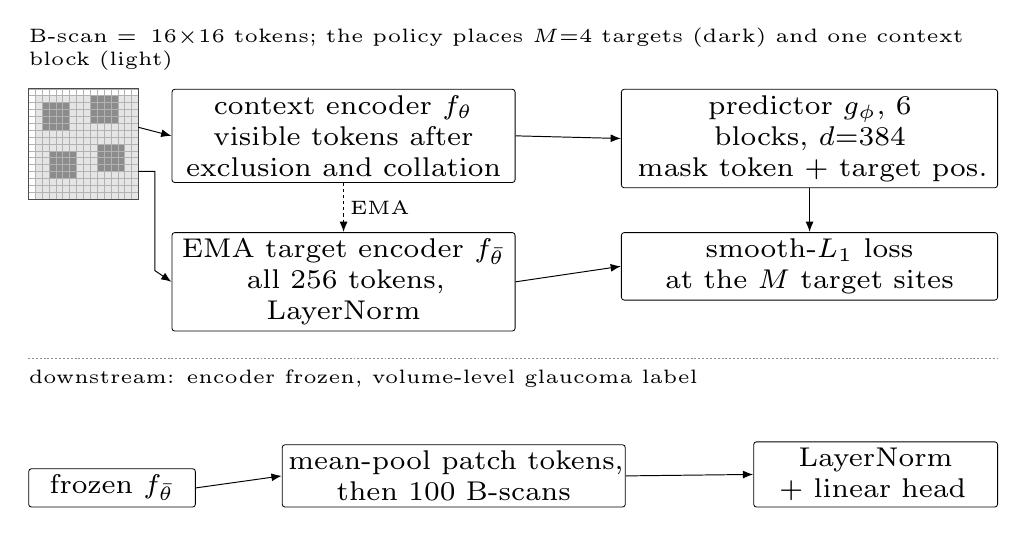
\begin{tikzpicture}[scale=1.4,transform shape,x=1mm,y=1mm,font=\scriptsize,
  bx/.style={draw,rounded corners=1pt,align=center,inner sep=1.6pt,line width=0.3pt},
  ar/.style={-{Latex[length=1.3mm,width=1.0mm]},line width=0.35pt},
  dr/.style={ar,dashed,dash pattern=on 1.1pt off 1.1pt}]
\node[anchor=south west,align=left,inner sep=0pt,text width=88mm,font=\tiny] at (0,39.6)
  {B-scan $=16{\times}16$ tokens; the policy places $M{=}4$ targets (dark) and one context block (light)};
% token grid: light cells are the context block, dark cells the M targets
\begin{scope}[shift={(0,28)}]
  \fill[black!10] (0.625,0) rectangle (10,9.375);
  \fill[black!45] (1.25,6.25) rectangle (3.75,8.75);
  \fill[black!45] (5.625,6.875) rectangle (8.125,9.375);
  \fill[black!45] (1.875,1.875) rectangle (4.375,4.375);
  \fill[black!45] (6.25,2.5) rectangle (8.75,5);
  \draw[step=0.625,black!30,line width=0.08pt] (0,0) grid (10,10);
  \draw[black!70,line width=0.3pt] (0,0) rectangle (10,10);
\end{scope}
\node[bx,anchor=north west,text width=30mm] (ctx) at (13,38) {context encoder $f_\theta$\\visible tokens after\\exclusion and collation};
\node[bx,anchor=north east,text width=33mm] (prd) at (88,38) {predictor $g_\phi$, 6 blocks, $d{=}384$\\mask token $+$ target pos.};
\node[bx,anchor=north west,text width=30mm] (tgt) at (13,25) {EMA target encoder $f_{\bar\theta}$\\all 256 tokens, LayerNorm};
\node[bx,anchor=north east,text width=33mm] (loss) at (88,25) {smooth-$L_1$ loss\\at the $M$ target sites};
\draw[ar] (10,34.5) -- (ctx.west);
\draw[ar] (10,30.5) -- (11.5,30.5) -- (11.5,21.5) -- (tgt.west);
\draw[ar] (ctx.east) -- (prd.west);
\draw[ar] (tgt.east) -- (loss.west);
\draw[ar] (prd.south) -- (loss.north);
\draw[dr] (ctx.south) -- node[right,inner sep=1.5pt,font=\tiny] {EMA} (tgt.north);
% downstream probe
\draw[black!45,dashed,dash pattern=on 0.7pt off 0.7pt,line width=0.25pt] (0,13.5) -- (88,13.5);
\node[anchor=west,inner sep=0pt,font=\tiny] at (0,11.7) {downstream: encoder frozen, volume-level glaucoma label};
\node[bx,anchor=south west,text width=14mm] (fr) at (0,0) {frozen $f_{\bar\theta}$};
\node[bx,anchor=south west,text width=30mm] (mp) at (23,0) {mean-pool patch tokens,\\then 100 B-scans};
\node[bx,anchor=south east,text width=21mm] (hd) at (88,0) {LayerNorm\\$+$ linear head};
\draw[ar] (fr.east) -- (mp.west);
\draw[ar] (mp.east) -- (hd.west);
\end{tikzpicture}
\caption{I-JEPA pretraining and frozen-encoder evaluation. The grid is schematic:
dark cells are target positions and light cells the candidate context. After
exclusion and collation, retained context tokens enter the online encoder.
The predictor uses target positions to regress features from the full-image
EMA target encoder; target-encoder gradients are stopped. Below the dashed
line, the frozen target encoder supplies patch features pooled into one
volume-level classification input. Source-verified token-map examples are
shown in Figure~\ref{fig:policies5}.}
\label{fig:policies}
\end{figure}

\subsection{Hypotheses}

We distinguish three hypotheses, the third of which requires stronger controls
than the present policy comparisons provide:

\begin{description}
\setlength{\itemsep}{1pt}\setlength{\parskip}{0pt}
\item[H1] \emph{Tissue-directed placement helps.} \textsc{envelope} $>$ \textsc{random}.
\item[H2] \emph{Anatomical precision helps further.} anatomy arms $>$
  \textsc{envelope}.
\item[H3] \emph{Any benefit is due to anatomical targeting, not to incidental
  changes in mask area, target count, or context size.}
\end{description}

\section{Experimental setup}
\label{sec:setup}

\paragraph{Data.} FairVision~\citep{luo2024fairvision} glaucoma OCT volumes.
Each volume is a 3D scan resampled to 100 B-scans of $256{\times}256$ after
transform. The label is a binary glaucoma diagnosis. Splits are fixed and
patient-disjoint as released. Downstream evaluation uses a held-out test split of
$N{=}3000$ volumes (1466 positive / 1534 negative), seed 42, fixed loader order.
No test volume is used to fit or select the probe head, which is selected on a
separate validation split. The study's choices of policy, checkpoint, analysis
and stopping horizon were made after repeated inspection of that same test split
(Section~\ref{sec:limits}). Test files are read in deterministic sorted order.
The saved label vectors agree across arms, but those vectors alone do not prove
case identity because the historical prediction files omit subject identifiers.
Paired analyses rely on the documented shared split and loader ordering.
Demographic attributes are used only for the subgroup
analysis in Section~\ref{sec:subgroup} and never as model inputs.

\paragraph{Pretraining.} Patch-level I-JEPA, ViT-Base, $256{\times}256$ crops,
patch size 16, predictor depth 6, EMA target encoder. The reference fork is the
epoch-25 checkpoint, with matched nominal optimiser, learning-rate and
weight-decay schedules and effective batch size (512).
The checked-in \textsc{anatomy-v1} configuration instead resumes an
\textsc{envelope} epoch-27 checkpoint; its exact historical launch record is
not retained, so a direct epoch-25 fork is not independently established for
that early result. Guidance is ramped linearly from epoch 25 to 30 and held at full strength
thereafter. Within the rectangle family the \emph{only} difference between arms
is the mask sampler (Section~\ref{sec:policies}). The anatomy family
also differs in collation, and
we quantify that in Section~\ref{sec:results}.

Arms differ in how far they were carried.
\textsc{random}, \ArmBest{} and \textsc{envelope} reach epoch 100.
\textsc{anatomy-v2} reaches epoch 75 (its epoch-75 and epoch-92 probes under an
earlier target-precision splice are excluded and replaced by a clean fp32
continuation, Appendix~\ref{app:excluded}). We stopped that arm having seen its
epoch-75 deficit, which is a selective stopping horizon and a real weakness:
a trajectory can recover, and its epoch-100 value is unmeasured, not known to be
worse.
\textsc{anatomy-v1} has only epoch 30. \textsc{cover} $f{=}0.21$ reaches epoch
100, with an extra probe at its epoch-73 peak. Epoch 50 is therefore the only
epoch at which
five policies are simultaneously available, and it carries every cross-policy
comparison that involves the anatomy or coverage arms.

\paragraph{Evaluation.} The frozen encoder is the EMA target branch, not the
online context encoder. Per-slice features are
mean-pooled over the volume, followed by LayerNorm and a linear head. The head is
selected by validation AUC and reported on the held-out test split. We report
percentile bootstrap intervals for primary AUCs and paired deltas (\Nboot{}
class-stratified subject resamples; fitted heads fixed and each draw shared across arms) and
DeLong tests for correlated ROC curves~\citep{delong1988roc}, both of which are
conditional on the shared case ordering of the documented evaluation loaders.
The historical archives contain matching labels but no independent case-ID
manifest, as noted above.
Each test volume is a distinct subject, so case-level resampling is already
subject-level and no cluster correction is
required~\citep{obuchowski1997clusteredroc,rutter2000clusterbootstrap}. We follow
\citet{maierhein2024metricsreloaded} in reporting the operating-point metrics
alongside AUC rather than AUC alone (Appendix~\ref{app:operating}).

\paragraph{Numerical precision.} The probe harness
defaults to mixed precision. The \textsc{random}, \ArmBest{} and
\textsc{envelope} long-horizon probes were fitted under that default (fp16).
The \textsc{anatomy-v1}, \textsc{anatomy-v2}, \textsc{cover} and ancestor probes
were fitted with autocast explicitly disabled (fp32). Protocol is therefore not
uniform across probes, so we partition the comparisons: all headline contrasts in
Table~\ref{tab:main} are drawn from arms sharing both epoch \emph{and}
precision, and any contrast that would cross the precision boundary is marked
as such and excluded from headline claims. Section~\ref{sec:precision} measures
the precision effect.

\section{Results}
\label{sec:results}

The tissue-directed rectangle policies improve AUC in these runs. The causal
effect of anatomical coverage is not identified here. Each policy was pretrained once, so the
intervals below are sampling error over test subjects, not seed-to-seed
variance (Section~\ref{sec:limits}).

\subsection{Tissue-directed rectangle placement improves the observed AUC}

\begin{table}[t]
\centering
\caption{Frozen MeanPool probe, FairVision test ($N{=}\Ntest$, \Npos{} positive).
The reference ancestor is epoch 25 (AUC $\AUCAncestor$); continuation provenance
is described in Section~\ref{sec:setup}. $\Delta$ is
versus \textsc{random} at the \emph{matched} epoch. The upper block is
precision-matched (fp16 throughout) and carries every headline claim; the lower
block is fp32, each $\Delta$ taken against an fp32 null re-probed at the same
epoch. The measured fp16/fp32
gap is at most $2\times10^{-4}$ (Appendix~\ref{app:fp32}).}
\label{tab:main}
\footnotesize
\setlength{\tabcolsep}{4pt}
\begin{tabular}{llcccccc}
\toprule
& & \multicolumn{2}{c}{epoch 50} & \multicolumn{2}{c}{epoch 75} & \multicolumn{2}{c}{epoch 100} \\
\cmidrule(lr){3-4}\cmidrule(lr){5-6}\cmidrule(lr){7-8}
policy & guidance signal & AUC & $\Delta$ & AUC & $\Delta$ & AUC & $\Delta$ \\
\midrule
\textsc{random}   & none (null)                      & \AUCRandomEpFifty  & ---                              & \AUCRandomEpSeventyFive  & ---                              & \AUCRandomEpHundred  & ---  \\
\textsc{envelope} & segmenter (location only)        & \AUCEnvelopeEpFifty & $\mathbf{\DEnvelopeRandomEpFifty}$ & \AUCEnvelopeEpSeventyFive & $\mathbf{\DEnvelopeRandomEpSeventyFive}$ & \AUCEnvelopeEpHundred & $\mathbf{\DEnvelopeRandomEpHundred}$ \\
\ArmBest{}   & intensity centroid, no segmenter & \AUCOracleEpFifty   & $\mathbf{\DOracleRandomEpFifty}$   & \AUCOracleEpSeventyFive   & $\mathbf{\DOracleRandomEpSeventyFive}$   & \textbf{\AUCOracleEpHundred} & $\mathbf{\DOracleRandomEpHundred}$ \\
\midrule
\textsc{anatomy-v2} & segmenter (target shape) & \TAUCAnatomyTwoEpFifty & \TAnatomyTwoRandomEpFifty & \TAUCAnatomyTwoEpSeventyFive & \TAnatomyTwoRandomEpSeventyFive & \TAUCAnatomyTwoEpHundred & \TAnatomyTwoRandomEpHundred \\
\textsc{cover} $f{=}.21$ & segmenter (coverage) & \TAUCCoverEpFifty & \TCoverRandomEpFifty & \TAUCCoverEpSeventyFive & \TCoverRandomEpSeventyFive & \TAUCCoverEpHundred & \TCoverRandomEpHundred \\
\bottomrule
\end{tabular}
\end{table}


\textbf{The observed comparisons are consistent with H1 in these continuations.}
\textsc{envelope} changes rectangle placement relative to the unguided
baseline (Section~\ref{sec:policies}). Delivered context also changes
($24.7\%$ to $30.7\%$, Table~\ref{tab:delivered}), so this comparison does
not isolate location from its consequences for the prediction task.
The AUC difference is
$\DEnvelopeRandomEpFifty$ AUC at epoch 50, and \ArmBest{}, a band located from
a first-order intensity statistic with no segmentation model anywhere, is worth
$\DOracleRandomEpHundred$ at epoch 100. Every \textsc{envelope} and \ArmBest{}
interval excludes zero at all three epochs, and all six contrasts survive
Benjamini--Hochberg correction over that family of nine ($q \leq
\DEnvelopeRandomEpHundredQ$; Figure~\ref{fig:traj}b, with the full paired
inference on all nine precision-matched contrasts in
Table~\ref{tab:contrasts}, Appendix~\ref{app:contrasts}).

Aiming is not containment: the rectangles are large, so fewer than half of
\textsc{envelope}'s masked cells land on tissue (Table~\ref{tab:geom}). Guidance
changes where the predictor is repeatedly sent, not what it is forbidden to see.
Background diagnostics provide a complementary view of the prediction task,
not an identified explanation of the AUC differences (Section~\ref{sec:results-bg}).

\begin{figure}[t]
\centering

\includegraphics[width=0.71\linewidth]{fig_trajectories_ci.png}
\caption{\textbf{(a)} Frozen-probe test AUC against pretraining epoch; note the
truncated AUC axis. The open star marks the shared epoch-25 ancestor.
Solid lines are the
precision-matched fp16 family; dashed lines are fp32
arms and must not be compared vertically against the solid lines.
\textbf{(b)} The actual inference: paired differences against the unguided null
on identical test cases, \Nboot-resample percentile bootstrap intervals. Every
\textsc{envelope} and \ArmBest{} interval excludes zero; \textsc{cover} straddles
zero at epoch 50 and is negative thereafter. Paired differences account for
the covariance of predictions on shared test cases; individual-arm intervals
answer a different question.}
\label{fig:traj}
\end{figure}

\textbf{The anatomy-shaped results are mixed.} H2 predicts that the anatomy arms exceed
\textsc{envelope}. Tested directly at the matched epoch 50, \textsc{anatomy-v2}
sits $\DAnatomyTwoEnvelopeEpFifty$ \emph{below} \textsc{envelope} (CI
$\DAnatomyTwoEnvelopeEpFiftyCI$). At epoch 30, however, \textsc{anatomy-v1} sits
$\DAnatomyOneEnvelopeEpThirty$ \emph{above} it (CI
$\DAnatomyOneEnvelopeEpThirtyCI$), with the early continuation's lineage
uncertainty described in Section~\ref{sec:setup}. These are different implementations at
different epochs, so we do not read either as settling H2. What the pair rules
out is a uniform observed ordering across these implementations, not a causal
effect of target shape. Neither \textsc{anatomy-v2} nor \textsc{cover} is resolved as
\emph{worse} than the null at the
matched epoch: both sit within a paired interval that comfortably contains zero
(Figure~\ref{fig:traj}b). Intervals containing zero do not establish equality
or exclude smaller beneficial or adverse effects.

\paragraph{Carried to epoch 100 the coverage arm degrades.}
\textsc{cover} is the only policy that uses the segmenter to choose \emph{how
much} to hide, and carried to the full horizon it produces the study's one
\emph{negative} result. It climbs normally to epoch 50, peaks at epoch
$\CoverPeakEpoch$, then \emph{falls}, losing $\DCoverPeakToHundred$ from its own
peak ($p\,\DCoverPeakToHundredP$) while the unguided null keeps improving
(Figure~\ref{fig:traj}). Its gap against the null widens monotonically across the
three matched epochs (Table~\ref{tab:main}).

We cannot read this as evidence that high coverage is harmful. An audit found
that the collator shortens predictor targets \emph{after} \textsc{cover} chooses
its placement, so its delivered masks hide \emph{less} anatomy than
\textsc{envelope}'s (Table~\ref{tab:geom}, Figure~\ref{fig:maskstats}) and the
arm never realised the coverage it was configured for.
Appendix~\ref{app:covbug} gives the full account.

\textbf{The strongest policy consults no segmentation model.} \ArmBest{} finds
its band from a per-column intensity centroid: no model and no annotation. Its
margin over the null is the largest at epoch 100 and does not decay with
training, whereas \textsc{envelope}'s does
(Table~\ref{tab:main}), and it exceeds the segmenter-guided \textsc{envelope} arm
at epoch 100 by $\DOracleEnvelopeEpHundred$ (CI $\DOracleEnvelopeEpHundredCI$),
though their paired intervals span zero at epochs 50 and 75.

\subsection{Delivered geometry limits the interpretation}
\label{sec:results-h3}

\begin{table}[t]
\centering
\caption{Measured mask geometry, 600 training slices, production samplers.
``purity'' is the fraction of masked cells lying on tissue; ``loss slots'' counts
supervised target-token instances, summed over the $M$ targets and including
duplicates. AUC is quoted at the
\emph{matched} epoch 50, so the geometry-to-AUC association is not read across
mixed epochs.}
\label{tab:geom}
\footnotesize
\begin{tabular}{lcccccc}
\toprule
policy & anatomy hidden & purity & mask ratio & context kept & loss slots & AUC @ep50 \\
\midrule
\textsc{random}   & 54.0\% & 31.5\% & 44.5\% & 41.9\% & 159.9 & \AUCRandomEpFifty \\
\ArmBest{}   & 62.1\% & 40.0\% & 40.3\% & 45.5\% & 159.0 & \AUCOracleEpFifty \\
\textsc{envelope} & 77.6\% & 43.3\% & 46.5\% & 40.6\% & 159.7 & \textbf{\AUCEnvelopeEpFifty} \\
\textsc{cover}    & 73.5\% & 44.2\% & 43.2\% & 43.2\% & 159.1 & \AUCCoverEpFifty \\
\textsc{anatomy-v2} & 79.9\% & \textbf{97.1\%} & 21.3\% & 67.7\% & 64.0 & \AUCAnatomyTwoEpFifty \\
\bottomrule
\end{tabular}
\end{table}

\textbf{The highest epoch-100 endpoint hides the least anatomy.} Of the four
guided arms the one
that hides the most (masking almost nothing but tissue, at $97.1\%$ purity)
does not separate from the null. Both readings come from running each
production sampler on 600 training slices and measuring the realised masks
(Table~\ref{tab:geom}, Figures~\ref{fig:paradox} and~\ref{fig:ladder};
provenance in Appendix~\ref{app:geomprov}). What \ArmBest{} does
instead is leave more visible: it retains more context than any other rectangle
arm, and the background stays maskable. Rank correlations over these
arms are positive for both anatomy hidden and purity, but at $n{=}4$--$5$ arms
they resolve nothing in either direction and we draw no inference from them.
Historical fine-tuned attribution images are not used to explain this result,
because their numerical inputs are not retained (Appendix~\ref{app:interp}).

\textbf{The anatomy arms are confounded on several axes simultaneously.}
\textsc{anatomy-v2} retains more context still, but it also hides far less of the
grid and collapses to
$64$ predictor loss slots against about $159$ for every rectangle arm
(Table~\ref{tab:geom}, Figure~\ref{fig:geom}), changing the prediction task. They and \textsc{cover}
also differ from \textsc{envelope} in guide provenance
(Appendix~\ref{app:repro}). Any of these could
account for its deficit without invoking target shape at all. \textbf{H3 is
therefore not identified by this design}, and we do \emph{not} claim that
irregular target shape is harmful.

These are not consequences of target shape: the anatomy arms resample
every target to a fixed $K{=}16$ cells, so $4\times16=64$ loss slots follows by
construction, while the rectangle arms do not set $K$. The two families are
collated differently, which weakens ``everything else held fixed'' for the
anatomy-versus-rectangle comparison specifically. Rectangle-family comparisons
share the collation rule but not necessarily its realized context or target
budgets (Appendix~\ref{app:covbug}).

\paragraph{Production-path replay.}
On fixed Training crops in full batches, historical \textsc{cover} loses
tissue targets through truncation in \DTTissueTruncation{} of \DTFullImages{}
views and leaves \DTZeroContext{} with no guide-positive encoder context.
Among \DTValidGuides{} valid guides, \DTLegacyFloorMiss{} miss the final
occupancy-cell context criterion defined in Appendix~\ref{app:delivered_audit}.
Scoring the exact delivered target prefixes removes
target-truncation losses but leaves \DTPrefixFloorMiss{} context-floor misses.
A separately enabled guide-aware context selection satisfies the floor in
these valid-guide cases. These measurements identify a mismatch between the
intended and delivered task, not the cause of the historical AUC ranking.
The corrected policies have not been pretrained; details and diagnostic
controls are in Appendix~\ref{app:delivered_audit}.

\subsection{Background targets and redundant downstream features}
\label{sec:results-bg}

Unguided masking often selects background targets. At epoch 100 the null's
predictor beats a per-position, no-context reference by $0.680$ on
\emph{background} targets, \emph{above} its $0.633$ on anatomy: predicting a
background token takes more than knowing where it sits, even though such tokens
start out nearly pure position ($90.8\%$ of across-position input variance there
comes from \texttt{pos\_embed}, against $40.8\%$ at tissue). Pretraining spends
self-similarity changes during training: under \textsc{envelope}, the one arm measured,
self-similarity falls from $0.784$ untrained to $0.346$.
In a separate epoch-50 regional probe using 25 slices and
2{,}000/600/1{,}000 training/validation/test volumes, pooled background features
are $95.2\%$ linearly reconstructible from pooled anatomy features.
Residualised, background
predicts glaucoma at test AUC $0.5515$ (barely above chance, though the
interval excludes it), and appending it to anatomy
\emph{lowers} test AUC for the null arm under that protocol. These diagnostics
show that predicting background embeddings is nontrivial and that their
incremental classification signal can be small. They do not establish why the
epoch-100 baseline is strong or whether background target selection causes a
downstream gain. The proposed causal controls were not run
(Appendix~\ref{app:bg}).

\subsection{A larger observed gap in low-label probe refits}
\label{sec:labeleff}

The observed margin is larger with fewer labels: at $5\%$ of the labelled set
($n{=}\LENFive$) \ArmBest{} leads the null by $\LEGapFive$, against
$\LEGapHundred$ at full supervision. This is descriptive evidence from
\LERepeats{} shared subset refits per low-label fraction, not a tested
gap-by-label-fraction interaction. Full-supervision fits agree with the
corresponding primary entries to within $0.0009$ across the four arms.
Appendix~\ref{app:labeleff} reports the curve, variation and protocol.


\subsection{Exploratory subgroup analysis}
\label{sec:subgroup}

Across seven stratifications and \NprobesSub{} probes spanning aggregate AUC
$\SubAUCMin$ to $\SubAUCMax$, the lowest-AUC group is unchanged for five
attributes. The metadata join uses deterministic loader order and reproduces
the saved labels; excluded probes remain excluded. These probes share a test
set and include multiple checkpoints from only \NbranchesSub{} branches,
so their subgroup rankings are descriptive, not independent replications.
The apparent checkpoint-level association between race gap and aggregate AUC
does not persist under branch aggregation (Appendix~\ref{app:subgroup}).

At epoch 100, \ArmBest{} has positive point-estimate gains in all race and
disease-severity strata shown, but the adjusted race intervals exclude zero
only for the white group. Severity strata are compared with the shared negative
pool; only the mild interval excludes zero after the declared family adjustment
(Tables~\ref{tab:severity} and~\ref{tab:pairedsub}). These results do not show
that one stratum benefits more than another. The paired difference between
gains in the lowest- and highest-AUC race groups is $\PDDiffRace$
(CI $\PDDiffRaceCI$); the corresponding gender contrast also includes zero.

No general equity improvement is established. Other attributes include
exceptions to the positive point-estimate pattern, and a shared validation-selected
threshold transfers unevenly across strata (Appendix~\ref{app:operating}).
The full subgroup and race-by-gender analyses are in
Appendices~\ref{app:subgroup} and~\ref{app:intersectional}. Masking policy is
not presented as a fairness intervention.

\subsection{Controls: the effect is not a precision artefact}
\label{sec:precision}

The eight recorded fp32 re-probes shift AUC by less than
$2\times10^{-4}$, orders of magnitude below the effects in
Table~\ref{tab:main}, so the differing autocast settings of
Section~\ref{sec:setup} are not the effect and every contrast is matched on
precision (Appendix~\ref{app:fp32}). The generating script, the epoch-100
\ArmBest{} encoder, its head and its stored per-case predictions are released
(links withheld for anonymity).
Re-encoding the test split from those weights on different hardware, at fp32
rather than fp16 and with a different encoder chunk size, reproduces the
reported AUC to $9.8\times10^{-6}$: 22
discordant pairs out of $2{,}248{,}844$.

\section{Discussion and limitations}
\label{sec:limits}

\paragraph{What the evidence supports.}
The segmenter-guided continuation has higher observed AUC by
$\DEnvelopeRandomEpFifty$ at epoch 50, and the intensity-centroid policy by
$\DOracleRandomEpHundred$ at epoch 100, relative to their matched uniform
baselines. Paired intervals exclude zero at all three observed epochs.
The latter policy requires no segmentation model. More anatomically specific
implementations do not have a consistent advantage, but this is not a controlled
test of target shape or coverage: delivered context, target area, loss weighting
and guide provenance differ. Background diagnostics motivate considering the
information in targets and context jointly, rather than treating all background
as wasted supervision. Their downstream causal contribution is unresolved.

\paragraph{What it does not support.}
We cannot claim anatomy-shaped masking is \emph{harmful}: at the matched epoch it
sits $\DAnatomyTwoRandomEpFifty$ from the null with an interval
($\DAnatomyTwoRandomEpFiftyCI$) that comfortably contains zero, so it is
not resolved as worse. Nor is target \emph{shape} identified as the
operative variable (Table~\ref{tab:geom}), nor is \ArmBest{}'s mechanism. Two
explanations remain live:
consistency of location (the encoder is repeatedly forced to represent the same
region), and masking ratio or task difficulty. Distinguishing them requires an
arm that randomises the band's vertical position while holding area and context
fixed, which we did not run.

\paragraph{One pretraining continuation per policy.}
The study uses a shared encoder ancestry and matched nominal training and probe
settings. The mask sampler is the intended
difference, though it also moves delivered mask ratio, retained context and loss
slots, and across families collation and guide provenance
(Section~\ref{sec:results-h3}). What it does not resample is pretraining
stochasticity, so each arm is one continuation.
The paired bootstrap bounds sampling error on a fixed test set, so the intervals
support statements about \emph{these} continuations rather than an expected
\emph{ranking} over retrainings, which pairwise significance on one test set does
not establish~\citep{bouthillier2021variance}. Probe-seed variance is outside the
design too: an earlier multi-seed probe check is not reproducible from retained
artifacts, so we state no bound on probe noise. A planned six-leg replication
is paused, with no completed epoch-50 replication result. It would add two
seeds each for \textsc{random}, \textsc{envelope} and \ArmBest{} from the
epoch-25 ancestor, under generated configurations differing in policy, seed
and logging fields. Seeds do not randomise the distributed sampler's visitation
order. The proposed analysis is recorded in Appendix~\ref{app:replication};
neither its existence nor a partial continuation increases the number of
completed runs in Table~\ref{tab:main}.

\paragraph{Scope, coverage and an incomplete arm.}
All results are glaucoma classification from FairVision OCT. Generality to other
modalities, diseases, or segmentation-quality regimes is untested, and the
anatomy arms depend on MIRAGE's prediction quality on this data, so a better
segmenter might change the conclusion. Only $f{=}0.21$ was pretrained for
\textsc{cover}, so we report no dose-response over the visible-tissue floor and
make no claim that any floor is optimal. That arm reaches epoch 100, but the
collation defect above (Appendix~\ref{app:covbug}) means its trajectory is not
evidence about aggressive coverage. Its epoch-50 value is retained as a
matched-epoch comparison against every other arm. Finally, one dataset and one test split were
reused throughout this programme's history, and policies, checkpoints and
analyses were chosen after repeated inspection of that split. The intervals we
report are therefore best read as descriptive rather than as confirmatory
inference.

\paragraph{Broader impact and ethics.}
This study uses a public, de-identified retinal dataset under its release terms
and involves no new recruitment or data collection, and no model reported here
is clinically validated or intended for deployment (Appendix~\ref{app:ethics}).

\section{Conclusion}

Tissue-directed rectangular target placement improves frozen-probe AUC in the
observed OCT continuations, including a simple segmentation-free centroid policy.
The results do not establish an equivalence between guidance methods or an
expected ranking across retrainings. More targeted masking is not a single
intervention when it also changes the context and target tokens delivered to
the model. The mixed anatomy-shaped results and the coverage implementation
defect therefore motivate joint control of target selection, retained context
and background supervision. Their causal contributions remain open. A
corrected, budget-matched multi-run comparison is subsequent work, not a result
implied by the present diagnostics.

\bibliographystyle{plainnat}
\bibliography{references}

\appendix

\section{All frozen probes}
\label{app:allprobes}

Table~\ref{tab:allprobes} lists every frozen MeanPool probe in the study. It has
37 rows: \Nprobes{} valid probes, plus two probes excluded and four retracted
for the reasons in Appendix~\ref{app:excluded}. Two further counts follow from
those \Nprobes{}. Eight of them are fp32 re-probes of an encoder already probed
at fp16, and the subgroup audit collapses each such pair to the single encoder it
scores twice, leaving \NprobesSub{} distinct encoder--epoch units
(Section~\ref{sec:subgroup}); \NprobesRace{} of those carry a stored per-group
race summary. The two race analyses therefore run on
different subsets by construction: the gap-trend test in
Table~\ref{tab:subtrends} uses all \NprobesSub{} probes, since every one carries
a race \emph{gap}, while the scatter in Figure~\ref{fig:fair} needs a per-group
AUC for all three groups and so uses the \NprobesRace{} probes that have one.
The four that do not are \textsc{cover} at epochs 73, 75 and 100 and
\textsc{anatomy-v2} at epoch 75: each was probed after the per-group race
artifact was generated, and that artifact was not recomputed, so their absence
is one of artifact chronology and not a property of those runs, whose race gaps
are present and do enter the \NprobesSub{}-probe trend test.

\begin{table}[h]
\centering
\caption{Every frozen probe in the study, including runs excluded from the
analysis and the reasons. The probe protocol is otherwise the same for every
row (FairVision test $N{=}\Ntest$, seed 42, frozen encoder, MeanPool +
LayerNorm + Linear) and differs only in the precision column.
``Precision'' is the probe-time
numerical precision, inferred from the stored prediction dtype, and is distinct
from the pretraining target precision discussed in
Appendix~\ref{app:excluded}.}
\label{tab:allprobes}
\footnotesize
\begin{tabular}{lcccc}
\toprule
policy & epoch & precision & test AUC & 95\% CI \\
\midrule
\textsc{anatomy-v1} & 30 & fp32 & 0.8583 & [0.8450,\,0.8712] \\
\textsc{anatomy-v2} & 35 & fp32 & 0.8661 & [0.8531,\,0.8787] \\
\textsc{anatomy-v2} & 40 & fp32 & 0.8683 & [0.8553,\,0.8807] \\
\textsc{anatomy-v2} & 50 & fp32 & 0.8654 & [0.8522,\,0.8781] \\
ancestor & 25 & fp32 & 0.8487 & [0.8349,\,0.8621] \\
\textsc{cover} & 27 & fp32 & 0.8483 & [0.8346,\,0.8617] \\
\textsc{cover} & 30 & fp32 & 0.8522 & [0.8386,\,0.8654] \\
\textsc{cover} & 34 & fp32 & 0.8571 & [0.8437,\,0.8700] \\
\textsc{cover} & 50 & fp32 & 0.8643 & [0.8513,\,0.8768] \\
\textsc{cover} & 73 & fp32 & 0.8647 & [0.8517,\,0.8772] \\
\textsc{cover} & 75 & fp32 & 0.8639 & [0.8507,\,0.8763] \\
\textsc{cover} & 100 & fp32 & 0.8577 & [0.8443,\,0.8707] \\
\textsc{envelope} & 30 & fp32 & 0.8539 & [0.8405,\,0.8669] \\
\textsc{envelope} & 50 & fp16 & 0.8761 & [0.8635,\,0.8879] \\
\textsc{envelope} & 50 & fp32 & 0.8761 & [0.8635,\,0.8879] \\
\textsc{envelope} & 75 & fp16 & 0.8803 & [0.8677,\,0.8922] \\
\textsc{envelope} & 75 & fp32 & 0.8803 & [0.8677,\,0.8922] \\
\textsc{envelope} & 100 & fp16 & 0.8807 & [0.8683,\,0.8926] \\
\textsc{envelope} & 100 & fp32 & 0.8808 & [0.8683,\,0.8927] \\
\ArmBest{} & 50 & fp16 & 0.8740 & [0.8615,\,0.8862] \\
\ArmBest{} & 50 & fp32 & 0.8740 & [0.8614,\,0.8862] \\
\ArmBest{} & 75 & fp16 & 0.8836 & [0.8714,\,0.8955] \\
\ArmBest{} & 100 & fp16 & 0.8855 & [0.8735,\,0.8971] \\
\ArmBest{} & 100 & fp32 & 0.8853 & [0.8732,\,0.8971] \\
\textsc{random} & 50 & fp16 & 0.8641 & [0.8510,\,0.8769] \\
\textsc{random} & 50 & fp32 & 0.8641 & [0.8511,\,0.8769] \\
\textsc{random} & 75 & fp16 & 0.8723 & [0.8593,\,0.8849] \\
\textsc{random} & 75 & fp32 & 0.8723 & [0.8593,\,0.8849] \\
\textsc{random} & 100 & fp16 & 0.8746 & [0.8618,\,0.8869] \\
\textsc{random} & 100 & fp32 & 0.8745 & [0.8617,\,0.8868] \\
anatomy-v2 & 75 & fp32 & 0.8625 & \emph{excluded} \\
anatomy-v2 & 92 & fp32 & 0.8604 & \emph{excluded} \\
random & 30 & fp32 & 0.8558 & \emph{retracted} \\
random & 50 & fp32 & 0.8590 & \emph{retracted} \\
random & 75 & fp32 & 0.8612 & \emph{retracted} \\
random & 100 & fp32 & 0.8607 & \emph{retracted} \\
\bottomrule
\end{tabular}

\end{table}

\section{Continuation-level replication}
\label{app:replication}

\textbf{Status at submission: paused; no completed replication result.}
The first leg has a completed epoch-26 checkpoint and an incomplete epoch 27,
not an epoch-50 probe. What follows is the recorded design for subsequent work,
not additional evidence for the present comparisons.

\paragraph{Design.} Six continuations (\textsc{random}, \textsc{envelope} and
\ArmBest{}, each at two further seeds) resume from the same epoch-25 ancestor
used by every arm in this paper. The ancestor is locked by content: SHA-256
\texttt{e5ad5b0c2aadfa15449409786afbfa39d8b5405b699be8f02f2e540195e97e7b},
1{,}507{,}519{,}602 bytes, re-hashed immediately before each leg, and a mismatch
aborts the leg rather than continuing from an unverified starting point. The six
configurations are generated by a script that asserts they are identical outside
the mask curriculum except for the seed and logging fields. Each leg runs to
epoch 50 (the endpoint at which every arm already carries a frozen probe)
with the optimiser, cosine learning-rate, weight-decay and EMA schedules still
sized for 100 epochs, so the trajectory is the one this paper measures and not a
shorter, differently-scheduled substitute. Each completed leg is then probed
under the frozen-probe protocol of Section~\ref{sec:setup}, with the encoder
hashed before and after the probe. Together with the continuations reported
here, this yields three continuations per policy at a matched endpoint.

\paragraph{Recorded analysis plan.} (i) All nine epoch-50 continuation AUCs would be
reported in one table, whatever they show. No continuation is dropped for any
reason other than a documented crash, and a crash is reported. (ii) We report
the per-policy mean and full range, and the two paired-by-seed differences
\textsc{envelope}$-$\textsc{random} and \ArmBest{}$-$\textsc{random}, one per
seed. (iii) At three continuations we report point estimates and ranges only:
no $t$-test, no $p$-value and no confidence interval at the continuation level,
because a small set of continuations gives a limited account of training
variability. (iv) The
fixed-data-order caveat below is restated wherever the result is.

\paragraph{What the seed does and does not randomise.} The seed randomises
random-resized-crop draws, target and context block sampling (including the
\textsc{envelope} rejection sampler and the \ArmBest{} band sampler), dropout,
and worker streams. It does \emph{not} randomise the order in which slices are
visited: the distributed sampler is constructed with its own fixed seed and
advanced per epoch, which is true of the originally reported continuations as
well. The unit of inference is therefore post-fork stochastic optimisation noise
at a fixed data order, which is narrower than independent retraining, and it is
not a replication of the data pipeline.

\paragraph{The failure case, written in advance.} If the epoch-50 ordering does
not reproduce (a paired difference changes sign, or the three-continuation
range for either contrast spans zero), the reported conclusion becomes that
the single-continuation contrasts of Table~\ref{tab:main} describe those
particular runs and not the policies, and every policy-level statement in this
paper is downgraded to a run-level one. Table~\ref{tab:main} is not withdrawn in
that case: it remains a correct description of the runs it measures. That
outcome is an anticipated and informative result of this design rather than a
failure of it, which is why the rules above are fixed now.

\paragraph{What this replication does not do.} It does not supply an untouched
evaluation cohort. The comparison still runs on the same test split, which has
been inspected repeatedly across this programme, so the replication bounds
run-to-run variability and not adaptive selection. The number of times that
split was inspected while choosing policies, checkpoints and analyses was not
logged and cannot now be reconstructed, which is why every interval in this
paper is described as descriptive rather than confirmatory. An untouched
evaluation would
require a labelled cohort from a different scanner or population, thresholds and
checkpoints selected on that cohort's own validation split, a single evaluation,
and no iteration afterwards. No such cohort was available to us.

\section{Masking policies across the volume}

\begin{figure}[h]
\centering

\includegraphics[width=\linewidth]{figS5_mask_statistics.png}
\caption{What each sampler actually does, measured on the 6,137-slice sweep
(\textsc{anatomy-v2} on $n{=}1{,}534$). Panel (a) is the quantity the
\textsc{cover} arm was built to maximise: it reaches $73.1\%$, \emph{below}
\textsc{envelope}'s $77.6\%$, which is the discrepancy Appendix~\ref{app:covbug}
explains. Panel (b) shows the ordering this paper tests: target purity
rises monotonically from \textsc{random} to \textsc{anatomy-v2}, while downstream
AUC does not follow it. Panels (c)--(f) give the confounds we do not
disentangle: how much anatomy survives in the context (c, d), the context
budget (e), and
how often a slice is left with no anatomy visible at all (f). Every bar starts
at zero and is a mean over the sweep, with no interval drawn; panel scales
differ, so bars should be compared only within a panel.}
\label{fig:maskstats}
\end{figure}

Figure~\ref{fig:policies5} compares final target and context sets on one
predeclared view. It illustrates the implementations, not population stability
across depth. The tissue reference and colour assignment are shared.

\begin{figure}[p]
\centering

\includegraphics[width=\linewidth]{fig_policy_family_token_maps.png}
\caption{Delivered token sets for five policy families on the first predeclared
Training view in the frozen two-view engineering-audit fixture. Orange cells
are the union of final predictor targets, hatched blue cells are final encoder
context, and hollow circles mark occupancy-guide-positive cells; other cells
are neither target nor context. The guide is a tissue proxy, not clinical ground
truth. All panels use the same input view and the already stored masks, without
redrawing seeds or displaying raw OCT pixels. ANATOMY-v2 represents the shaped
family, not ANATOMY-v1; COVER shows the historical implementation, not the proposed
correction. Placements are not exactly paired across policies, and unions do not
show repeated loss slots. This selected engineering example is not a population
summary or evidence of downstream performance.}
\label{fig:policies5}
\end{figure}

\section{Mask-geometry provenance}
\label{app:geomprov}

Table~\ref{tab:geom} was regenerated from the production samplers rather than
carried forward from an earlier draft, and this appendix records how, together
with two facts the table itself cannot show: how much of each cell is
measurement noise, and how one configuration constant moves the correlation
quoted in Section~\ref{sec:results-h3}.

\paragraph{How the geometry was measured.} Each production sampler was run on
the same 600 FairVision \emph{Training} slices (24 volumes, 25 slices each),
one image at a time, with the \textsc{cover} visible-tissue floor at its
production value $f{=}0.21$, on the $16\times16$ patch grid, with anatomy taken
from the MIRAGE guide occupancy channel at threshold $0.25$. The measurement was
repeated with three independent draws (seeds 42, 1234 and 2026). Training slices
are not a choice: the cached anatomy guides exist for the Training split only,
so three of the five production samplers cannot be run on held-out slices at
all.

\paragraph{Cell-level agreement and seed noise.} Table~\ref{tab:geom} now carries
the regenerated values, so the question is how stable they are across draws.
18 of the 25 cells fall inside the three-seed range of the measurement and do
not exceed observed re-draw variation. Across the four rectangle arms the
\emph{loss slots} spread is smaller than the per-arm seed spread
(Table~\ref{tab:geomprov}), so that column's ordering carries no information and
no claim in this paper depends on it. The rank order of the arms on anatomy
hidden and on purity is identical across all three draws, which is what the
rank correlations in the main text rely on.

\begin{table}[h]
\centering
\caption{Stability of two Table~\ref{tab:geom} columns across three independent
draws of the same 600-slice measurement. ``sd'' is the standard deviation over
seeds 42, 1234 and 2026. The loss-slot differences between rectangle arms are
smaller than this noise.}
\label{tab:geomprov}
\small
\begin{tabular}{lcccc}
\toprule
 & \multicolumn{2}{c}{anatomy hidden (\%)} & \multicolumn{2}{c}{loss slots} \\
\cmidrule(lr){2-3}\cmidrule(lr){4-5}
policy & value & sd & value & sd \\
\midrule
\textsc{random}     & 53.95 & 0.71 & 159.91 & 1.15 \\
\ArmBest{}          & 62.13 & 0.64 & 158.99 & 0.43 \\
\textsc{envelope}   & 77.58 & 0.38 & 159.68 & 1.00 \\
\textsc{cover}      & 73.55 & 0.30 & 159.09 & 0.45 \\
\textsc{anatomy-v2} & 79.89 & 0.39 & 64.00  & 0.00 \\
\bottomrule
\end{tabular}
\end{table}

\paragraph{The delivered context is not the per-image context.} The ``context
kept'' column of Table~\ref{tab:geom} is per-image geometry, measured before
collation. In training, every context mask in a batch is truncated to the batch
minimum, so what the encoder actually receives at the production batch size is
smaller, and unevenly so (Table~\ref{tab:delivered}). The context confound
between the anatomy arm and the rectangle arms that
Section~\ref{sec:results-h3} declines to explain
away is consequently \emph{larger} than the printed table suggests: roughly a
doubling rather than a $1.6\times$ ratio. This strengthens the verdict that H3
is not identified by this design.

\begin{table}[h]
\centering
\caption{Visible context as a fraction of the patch grid, same 600 slices and
same seed, measured per image and as delivered to the encoder at the production
batch size of 64. The per-image column reproduces
Table~\ref{tab:geom}'s ``context kept'' to within $0.4$ points.}
\label{tab:delivered}
\small
\begin{tabular}{lcc}
\toprule
policy & per image & delivered at batch 64 \\
\midrule
\textsc{random}     & 41.9\% & 24.7\% \\
\ArmBest{}          & 45.5\% & 32.9\% \\
\textsc{envelope}   & 40.6\% & 30.7\% \\
\textsc{cover}      & 43.2\% & 30.1\% \\
\textsc{anatomy-v2} & 67.7\% & 63.5\% \\
\bottomrule
\end{tabular}
\end{table}

\paragraph{The rank correlation depends on a configuration constant.} The
$+0.80$ anatomy-hidden/AUC Spearman coefficient of
Section~\ref{sec:results-h3} is computed at the production \textsc{cover} floor
$f{=}0.21$. Re-measured on the same slices with the floor at $0.15$,
\textsc{cover} hides $79.5\%$ of anatomy instead of $73.4\%$ at the same batch
size and overtakes
\textsc{envelope}, which reorders the four rectangle arms and moves the same
coefficient to $+0.40$. A rank statistic over four arms that a single
configuration constant can move by that much is not evidence about anatomy, in
either direction, which is why Section~\ref{sec:results-h3} draws its conclusion
from the direct comparison instead.

\paragraph{What would identify target shape.} An arm that isolated target shape
would have to match \textsc{envelope} on the axes that currently differ, and
those requirements are numeric, not rhetorical. \textsc{anatomy-v2} sets four
predictor targets resampled to a fixed $K{=}16$ cells, giving exactly 64 loss
slots. Matching the rectangle arms' $158$--$160$ slots at four targets requires
$K\approx40$ (inferred arithmetic on those measured values). It would also have
to deliver a mask ratio of $40$--$46\%$ of the grid rather than the $21\%$ that
the anatomy arms deliver, roughly twice the target area, which for a
shape-following sampler means more or larger connected components and therefore changes the
very shape statistics being tested, and it would have to pass through the
rectangle collation path, including the batch-minimum truncation above. It would
then need the same replicated continuation design and the same endpoint as
Appendix~\ref{app:replication}. We did not run it. Naming its specification is
what we can offer instead.

\section{Subgroup and severity analysis}
\label{app:subgroup}

\begin{figure}[h]
\centering

\includegraphics[width=\linewidth]{fig_fairness.png}
\caption{\textbf{Left:} race-stratified AUC at epoch 100. Points are group AUCs
and vertical bars are 3{,}000-resample class-stratified percentile bootstrap
intervals within each group, with fitted heads fixed and
per-group $n$ in the legend. The black subgroup is lowest under every policy, yet
\emph{every} group point estimate rises from \textsc{random} to \ArmBest{}.
\textbf{Right:} max--min race gap against aggregate AUC, one point per probe
over the \NprobesRace{} probes that carry a race summary; the legend keys colour
and marker to policy. The dashed line is a
least-squares fit while the quoted correlation is Spearman. The slope is
positive but fails multiplicity correction at
checkpoint level and does not survive branch-level aggregation
(Table~\ref{tab:subtrends}), so we draw no trend conclusion from it.}
\label{fig:fair}
\end{figure}

All numbers below come from saved test predictions joined to FairVision's
released metadata in deterministic loader order. The join is validated by exact
label reconstruction (\Ntest/\Ntest{} labels recovered in every probe). The
\NprobesSub{} probes used here are exactly those the inventory marks valid: the
four retracted \textsc{random} probes of Appendix~\ref{app:excluded} and the two
precision-spliced \textsc{anatomy-v2} probes are excluded here as everywhere
else in the paper.

\paragraph{Missing data.} No case is dropped for a missing attribute anywhere in
this paper and no value is imputed, so the per-group denominators sum to the full
test split rather than to a complete-case subset. The released metadata carries
every attribute we use for all \Ntest{} test subjects, whose identifiers are all
distinct, and the label is complete at \Npos{} positive and \Nneg{} negative.
Race is \NAsian{} asian, \NBlack{} black and \NWhite{} white; gender is 1{,}716
female and 1{,}284 male; ethnicity is 2{,}894 non-hispanic and 106 hispanic;
language is 2{,}782 english, 174 other and 44 spanish; marital status is 1{,}741
married or partnered, 776 single, 199 widowed, 191 divorced, 71 unknown and 22
legally separated; age is present and numeric for all \Ntest{}, spanning
$9.5$--$98.0$ years. Each of those five categorical breakdowns sums to \Ntest{}
exactly, which is the check a reader should apply to the tables below.

One level is non-substantive rather than absent: 71 of \Ntest{} subjects
($2.4\%$) carry marital status \emph{unknown} in the release. We keep it as its
own category rather than dropping those subjects or folding them into a
substantive group, so it is subject only to the same underpowering rule as every
other level. Severity is derived from visual-field mean deviation, and its 334
severe, 460 moderate and 672 mild strata sum to all \Npos{} positives, so no
positive is lost at a stratum boundary. The release uses a mean-deviation
sentinel of $-1$ in 3 of the \Ntest{} test records. All 3 carry a negative label,
and because every severity stratum is scored against the undifferentiated pool of
all \Nneg{} negatives, that sentinel never enters a stratum definition.

Separately from missingness, a group with fewer than 50 cases, or fewer than 10
of either class, is still computed and reported but is marked underpowered and
held out of the max--min gap summaries. That is an exclusion from the fairness
claim, not from the data, and it is the only place a group is set aside.

\paragraph{Why we report two sample sizes.} The \NprobesSub{} probes span only
\NbranchesSub{} pretraining branches, because several are different epochs of
one training run. Probes within a branch share an encoder lineage, a seed and
the test split, so treating them as \NprobesSub{} independent observations is
pseudo-replication. Table~\ref{tab:subtrends} therefore reports each trend twice:
once per checkpoint, and once after averaging within each branch. Where the two
disagree, the branch-level figure is the one to believe.

\begin{table}[h]
\centering
\caption{Subgroup gap trends. ``gap range'' is the max--min subgroup AUC gap
observed across the \NprobesSub{} valid probes. $q$ is Benjamini--Hochberg
across the seven checkpoint-level tests. Branch $p$-values are unadjusted across
the same seven and, at $n{=}7$, descriptive only. Only gender survives checkpoint-level
correction at the conventional $0.05$ level, and it
\emph{narrows} as aggregate AUC rises. Race, ethnicity and disease severity share
the same $q$ just above that level, so no threshold admits race and severity
without also admitting ethnicity. Race is the one attribute whose
checkpoint-level trend does not
persist under branch aggregation ($p{=}0.4821$), where the effective sample is
\NbranchesSub{} independent branches rather than \NprobesSub{} probes; we
therefore draw no trend conclusion for race.}
\label{tab:subtrends}
\footnotesize
\setlength{\tabcolsep}{4pt}
\begin{tabular}{llccccccc}
\toprule
& & & \multicolumn{3}{c}{per checkpoint ($n{=}27$)} & \multicolumn{2}{c}{per branch ($n{=}11$)} \\
\cmidrule(lr){4-6}\cmidrule(lr){7-8}
attribute & worst group & gap range & $\rho$ & $p$ & $q$ & $\rho$ & $p$ \\
\midrule
sex & female (27/27) & 0.0270--0.0396 & -0.739 & $<$0.0001 & $<$0.0001 & -0.891 & 0.0002 \\
race & black (27/27) & 0.0433--0.0935 & +0.487 & 0.0100 & 0.0232 & +0.518 & 0.1025 \\
ethnicity & hispanic (27/27) & 0.0203--0.0661 & +0.151 & 0.4509 & 0.4509 & +0.409 & 0.2115 \\
language & other languages (22/27) & 0.0518--0.0805 & +0.184 & 0.3589 & 0.4187 & +0.400 & 0.2229 \\
marital status & single (27/27) & 0.0349--0.0654 & -0.380 & 0.0503 & 0.0881 & -0.373 & 0.2589 \\
age & $<$60 (26/27) & 0.0474--0.0704 & +0.300 & 0.1279 & 0.1791 & +0.236 & 0.4841 \\
disease severity & mild ($-6$,$-2$] (27/27) & 0.1266--0.1400 & -0.551 & 0.0029 & 0.0102 & -0.618 & 0.0426 \\
\bottomrule
\end{tabular}

\end{table}

\paragraph{Race.} The black subgroup has the lowest AUC in every one of the
\NprobesSub{} probes ($n{=}\NBlack$ black, $n{=}\NAsian$ asian, $n{=}\NWhite$
white; Figure~\ref{fig:fair}). At matched epoch 100 the black subgroup improves from
$\RaceRandomBlack$ under \textsc{random} to $\RaceOracleBlack$ under
\ArmBest{} ($\BlackGainOracle$), a larger absolute gain than the white
subgroup's ($\RaceRandomWhite \to \RaceOracleWhite$). The max--min gap
nonetheless widens slightly, because the asian subgroup (already the
highest) gains most ($\RaceRandomAsian \to \RaceOracleAsian$). A widening
max--min gap with universally rising subgroup AUCs is not evidence of harm. The
checkpoint-level correlation between aggregate
AUC and racial gap is $\rho{=}\SubRaceRho$ ($p{=}\SubRaceRhoP$). It does not
pass Benjamini--Hochberg correction at the stated conventional threshold
($q{=}\SubRaceQ$), and it vanishes once probes are aggregated to their
pretraining branches ($\rho{=}\SubRaceBranchRho$,
$p{=}\SubRaceBranchP$), and the checkpoint-level test is pseudo-replicated
because the \NprobesSub{} probes come from only \NbranchesSub{} branches.

\paragraph{Disease severity.} FairVision's label is defined by visual-field mean
deviation (md): every test volume with md $\leq -2$ is positive. Severity
therefore cannot be used as an ordinary subgroup axis, because within-bin AUC is
undefined, a trap that silently yields nothing under naive stratification.
Instead each positive stratum is scored against the shared pool of all
\Nneg{} negatives (Table~\ref{tab:severity}).

\begin{table}[h]
\centering
\caption{Severity-stratified AUC at matched epoch 100. Each positive stratum is
scored against the shared pool of all \Nneg{} negatives. Each point estimate rises;
the gains were not tested against one another.}
\label{tab:severity}
\small
\begin{tabular}{lccccc}
\toprule
stratum & $n_{+}$ & \textsc{random} & \textsc{envelope} & \ArmBest{} & $\Delta$ \\
\midrule
severe (md $\leq -12$)          & 334 & \SevRandomSevere   & \SevEnvelopeSevere   & \SevOracleSevere   & \SevDeltaSevere \\
moderate ($-12 <$ md $\leq -6$) & 460 & \SevRandomModerate & \SevEnvelopeModerate & \SevOracleModerate & \SevDeltaModerate \\
mild ($-6 <$ md $\leq -2$)      & 672 & \SevRandomMild     & \SevEnvelopeMild     & \SevOracleMild     & \textbf{\SevDeltaMild} \\
\bottomrule
\end{tabular}
\end{table}

The severe-to-mild gap is $\SevGapRandom$ for the null and $\SevGapOracle$ for
the strongest policy, and stays within $\SeverityGapSpread$
($\SubSeverityGapMin$--$\SubSeverityGapMax$) across all \NprobesSub{} probes
while aggregate AUC spans $\SubAUCMin$--$\SubAUCMax$. All three point estimates
rise, but family-wise simultaneous adjustment leaves only mild excluding zero.
Moderate and severe no longer do (Table~\ref{tab:pairedsub}). The largest point estimate is at mild
disease ($\PDSevMildDelta$, CI
$\PDSevMildCI$) and the smallest at severe ($\PDSevSevereDelta$). That ordering
is descriptive only: we did not test the paired \emph{difference} between
strata, so it does not establish that mild disease benefits most. Mild
functional loss is harder to separate from normal OCT by construction, so
the difficulty ordering is expected clinically. What the data add is that no
masking policy we tested changes it.

\begin{table}[h]
\centering
\caption{Paired change in subgroup AUC from \textsc{random} to
\ArmBest{} at matched epoch 100. The eight rows plus two gain-difference
contrasts in the text form one exploratory family. Reported CIs are 95\%
single-step max-$|t|$ simultaneous intervals from \Nboot{} outcome-stratified
paired subject resamples shared across both fixed heads and every stratum
(family-wise $\alpha=0.05$). Four of ten exclude zero: mild severity, white
race, and both gender strata.}
\label{tab:pairedsub}
\small
\begin{tabular}{lcccc}
\toprule
stratum & $n$ & $\Delta$ AUC & 95\% CI & excludes 0 \\
\midrule
severity, mild & 2206 & +0.01372 & [+0.00541,\,+0.02192] & yes \\
severity, moderate & 1994 & +0.01016 & [+0.00262,\,+0.01757] & yes \\
severity, severe & 1868 & +0.00626 & [+0.00104,\,+0.01187] & yes \\
race, White & 2318 & +0.01129 & [+0.00518,\,+0.01731] & yes \\
race, Black & 431 & +0.01467 & [-0.00055,\,+0.03060] & no \\
race, Asian & 251 & +0.01558 & [-0.00079,\,+0.03283] & no \\
sex, Female & 1716 & +0.01152 & [+0.00412,\,+0.01890] & yes \\
sex, Male & 1284 & +0.01006 & [+0.00335,\,+0.01678] & yes \\
\bottomrule
\end{tabular}

\end{table}

\paragraph{Limitations.} The $p$-values here are descriptive, for the reasons
given in Section~\ref{sec:limits}. Race and ethnicity are
self-reported categories inherited from FairVision's coding. A race-by-gender
intersectional breakdown \emph{is} reported, in
Appendix~\ref{app:intersectional}. Its limits are that two of its six cells hold
fewer than $130$ cases and that it carries no paired per-cell intervals, so it
describes the disparity and tests no per-cell change.
All figures are frozen mean-pool
linear probes. Subgroup sensitivity, specificity and race-stratified expected
calibration error at a transferred threshold are reported in
Appendix~\ref{app:operating}. What is absent is subgroup predictive values,
reliability curves, and calibration stratified by any attribute other than race,
so this is not a complete fairness
evaluation. Disparities
could differ under fine-tuning or a stronger head.

\subsection{Intersectional breakdown: race by gender}
\label{app:intersectional}

The audit above crosses no attributes, so on its own it cannot say whether a
group disadvantaged on two axes at once is worse served than either margin
implies. We therefore also computed AUC for all six race-by-gender cells of the
test split, from the same saved predictions, under the same exact-label join
proof, with per-arm, 2{,}000-resample class-stratified percentile intervals
within each cell and fitted heads fixed. The second axis is FairVision's self-reported gender coding,
which we retain here without reinterpreting it as a biological-sex measure.
Legacy figures using ``sex'' refer to this same released variable.
The artifact behind this subsection
covers 22 arms, 18 of them non-retracted. Those 18 are a strict subset of the
\NprobesSub{} probes of Table~\ref{tab:subtrends}. Five are absent:
\textsc{cover} at epochs 50, 73, 75 and 100, and the \textsc{anatomy-v2}
epoch-75 probe, whose run directory carries the internal name \texttt{blob},
an artifact label for the anatomy-shaped family that this paper calls
\textsc{anatomy-v2}, and the only place that label survives here. All five were
probed after this
artifact was generated and it was not recomputed, so their absence is artifact
chronology rather than an analytic exclusion. The four retracted arms the
artifact does contain are dropped for the reasons in
Appendix~\ref{app:excluded}. Every count in this subsection is therefore
out of 18 arms, not \NprobesSub{}.

\begin{table}[h]
\centering
\caption{Race-by-gender AUC at matched epoch 100 on the \Ntest{} test volumes, with
per-cell counts and per-arm bootstrap percentile intervals. $\Delta$ is
\ArmBest{} minus \textsc{random} as a difference of point estimates. The
artifact stores per-arm intervals only and no paired per-cell resampling, so no
$\Delta$ in this table is tested against zero; per-cell significance is not reported.
The 18 intervals are marginal, not simultaneous.
The two asian cells are small ($n{=}123$ and $n{=}128$) and their intervals are
correspondingly wide.}
\label{tab:intersectional}
\scriptsize
\setlength{\tabcolsep}{3.5pt}
\begin{tabular}{lrrcccr}
\toprule
cell & $n$ & $n_{+}$ & \textsc{random} & \textsc{envelope} & \ArmBest{} & $\Delta$ \\
\midrule
asian $\times$ female & 123  & 52  & 0.8761 [0.8024, 0.9342] & 0.8762 [0.8042, 0.9366] & 0.8904 [0.8245, 0.9423] & $+0.0144$ \\
asian $\times$ male   & 128  & 66  & 0.9245 [0.8752, 0.9655] & 0.9145 [0.8565, 0.9626] & 0.9409 [0.8983, 0.9751] & $+0.0164$ \\
black $\times$ female & 250  & 149 & 0.8195 [0.7668, 0.8679] & 0.8155 [0.7632, 0.8638] & 0.8309 [0.7790, 0.8783] & $+0.0114$ \\
black $\times$ male   & 181  & 119 & 0.8435 [0.7822, 0.8994] & 0.8652 [0.8091, 0.9141] & 0.8663 [0.8132, 0.9149] & $+0.0228$ \\
white $\times$ female & 1343 & 610 & 0.8641 [0.8441, 0.8826] & 0.8728 [0.8530, 0.8910] & 0.8762 [0.8570, 0.8943] & $+0.0121$ \\
white $\times$ male   & 975  & 470 & 0.8864 [0.8650, 0.9062] & 0.8958 [0.8744, 0.9148] & 0.8962 [0.8746, 0.9153] & $+0.0099$ \\
\midrule
max$-$min gap         &      &     & 0.1050 & 0.0990 & 0.1100 & \\
\bottomrule
\end{tabular}
\end{table}

\paragraph{The ordering compounds, and it never reorders.} The black
$\times$ female cell has the lowest AUC in all 18 non-retracted arms and the
asian $\times$ male cell the highest in all 18. Within each race the female cell
sits below the male cell in all $54$ race-by-arm combinations, and within each
gender the black cell sits below the white cell in all $36$. These 18 arms share one
test split, one epoch-25 ancestor and one probe seed, and several are different
epochs of a single branch, so this unanimity is a consistency check across
checkpoints, not 18 replications. We attach no $p$-value to it, exactly as for
the marginal ordering above.

\paragraph{The marginal race gap understates the worst cell.} Averaged over the
18 arms, the max$-$min gap is $0.0340$ by gender alone, $0.0653$ by race alone, and
$0.1046$ across the six race-by-gender cells, and the intersectional gap exceeds
that arm's marginal race gap in all 18. The race margin therefore understates
the spread a race-by-gender reading exposes by $60.1\%$ on average, arithmetic on
those two means, not a separate measurement. The same pattern holds at the
matched epoch of Table~\ref{tab:intersectional}: under \ArmBest{} the marginal
race gap is $0.0717$ while the race-by-gender gap is $0.1100$, and the worst cell,
black $\times$ female at $0.8309$, sits $0.0163$ below the marginal black figure
$\RaceOracleBlack$ that the marginal audit above reports. An audit that stops
at the margins reports a worst-group number that is optimistic relative to the
worst cell. The compounding is close to additive and we do not claim more: the
gender and race means sum to $0.0993$ against an observed $0.1046$, a ratio of
$1.053$, which is not evidence of a super-additive interaction.

\paragraph{Not every cell improves.} The statement elsewhere in this appendix
that every subgroup point estimate rises from \textsc{random} to \ArmBest{} is a
statement about marginal strata at the matched epoch, and it does \emph{not}
extend to cells at every epoch. At epoch 100 all six point estimates rise
(Table~\ref{tab:intersectional}), but at epoch 50 the asian $\times$ female cell
falls by $0.0020$, and \textsc{envelope} minus \textsc{random} is negative in
three of six cells at epoch 75 (asian $\times$ female $-0.0148$, asian $\times$
male $-0.0031$, black $\times$ female $-0.0025$) and in two of six at epoch 100
(asian $\times$ male $-0.0100$, black $\times$ female $-0.0040$, with asian
$\times$ female at $+0.0001$). No policy we tested raises every intersectional
cell at every epoch, and the exceptions fall in the small asian cells and in the
worst cell.

\paragraph{What this does not establish.} There are no paired per-cell bootstrap
intervals in the artifact, so every $\Delta$ above is a difference of point
estimates and none of them is separated from zero. Per-cell delta significance
is not computed here, though it is computable from the retained per-arm
predictions. Two cells
carry $n{=}123$ and $n{=}128$, so their intervals overlap almost everything.
Cells with a single class or fewer than $40$ cases would have been dropped. None
were, so all six race-by-gender cells are reported. Nothing here is a fairness
intervention: as with the margins, no policy reorders the cells, and the
worst-served cell is the same under the unguided null and under every guided
policy we tested.

\section{Excluded runs}
\label{app:excluded}

Four probes of an earlier \emph{null} run are excluded from all analysis. They
are unguided-masking controls from a superseded coverage campaign: the
inventory lists them under \textsc{random}, and their run tags begin
\texttt{frozen\_cover\_random} because of that campaign, not because they use a
coverage policy. They were
trained with half-precision EMA targets and a different encoder-truncation
policy from the arms they would be compared against, so their deficit is not
attributable to masking. Similarly, the \textsc{anatomy-v2} probes at
epochs 75 and 92 follow a change of target precision partway through that arm's
training. They are listed in Table~\ref{tab:allprobes} but excluded from the
matched-epoch comparisons in Table~\ref{tab:main}.

\section{A collation defect in the coverage arm, and what it invalidates}
\label{app:covbug}

We audited the \textsc{cover} sampler after its epoch-100 result and found a
defect. It invalidates the reading of that arm and weakens one cross-family
comparison.

\paragraph{The defect.} Predictor targets are collated by truncating every target
to the length of the shortest target anywhere in the microbatch. \textsc{cover}
chooses its placement \emph{before} this happens: it greedily maximises hidden
anatomy subject to a visible-tissue floor, evaluated on full rectangles, and the
collator then shortens those rectangles. The optimisation is therefore defeated
after the fact.

\paragraph{Measured consequences.} A one-off audit found that collation reduced
\textsc{cover}'s anatomy coverage. An independent sweep over $6{,}137$ slices
gives $73.1\%$ against $77.6\%$ for \textsc{envelope}. The arm intended to hide
\emph{more} anatomy than \textsc{envelope} in fact hides \emph{less}. Across
$24{,}000$ emitted targets only $73.4\%$ remain perfect
rectangles. Because target cells are enumerated row-major, truncation keeps the
top of each rectangle and discards the bottom, so the loss is directional rather
than a neutral shrink. \emph{Provenance:} the one-off CPU audit of 194 accepted
slices that first exposed the defect was not persisted, so its pre- and
post-truncation figures are no longer asserted. The $73.1\%$ against $77.6\%$
comparison, which is the only figure the body relies on, is backed by the stored
floor sweep and is unaffected.

\paragraph{Why it went unnoticed.} Realised coverage is recorded before
truncation. Every training log therefore reported the intended figure, and the
instrument agreed with the design rather than with the data.

\paragraph{What it invalidates.} We cannot claim that \textsc{cover} tests
aggressive anatomy coverage, nor that its decline shows over-covering anatomy is
harmful. On delivered masks it does not out-cover \textsc{envelope}. Its measured
trajectory remains a real property of the policy as implemented. The mask
geometry in Table~\ref{tab:geom} is unaffected, having been measured on delivered
masks.

\paragraph{Scope.} \textsc{envelope} shares the same collation path and the same
directional clipping, but sets no exact coverage target, so it has no comparable
optimisation to defeat. The anatomy arms instead resample every target to a fixed
$K{=}16$ cells. Contrasts within the rectangle family are collated identically
and are unaffected. The anatomy-versus-rectangle contrast is not, and we treat it
accordingly in Section~\ref{sec:results}. A corrected coverage arm must be
retrained from the shared ancestor, since patching mid-trajectory would splice
two masking policies into one curve.

\paragraph{Status of a corrected run.} At submission the corrected arm is
\CoverFixedStatus{}. Until it exists, the question this arm was built to answer
(whether hiding most of the anatomy is harmful) remains \emph{open}.

\section{Delivered-task replay and versioned corrections}
\label{app:delivered_audit}

\paragraph{Scope.}
We replayed the actual guided dataset, paired transforms, DataLoader worker
collator and returned mask tensors on the existing 600-view Training scope
(24 volumes, 25 views each), using fixed new crop draws shared across policies.
These are not reconstructed historical training crops. Drawn block sizes were
injected independently of placement; equal seeds alone do not pair
policy-dependent rejection sampling. The production-size subset contains
\DTFullImages{} views in complete batches of 64, with \DTValidGuides{} valid
post-crop guides. The shorter final batch is excluded from
Table~\ref{tab:delivered_repair}. Views within volumes are correlated, so these
are descriptive engineering counts, not independent training replications.

\paragraph{What is measured.}
Target coverage is measured both at scoring and after target collation.
Encoder-visible tissue is counted only in the final encoder indices, not
in the full-grid target complement. Tissue is a guide occupancy thresholded
at $0.25$, not clinical ground truth. The context criterion is at least
$\max(\lceil 0.21N_{\mathrm{tissue}}\rceil,\min(4,N_{\mathrm{tissue}}))$
non-target tissue cells. It is an explicit occupancy-cell diagnostic and
corrected-policy guarantee, distinct from the historical soft-mass constraint
on the target complement.

\begin{table}[h]
\centering
\caption{Full-batch delivered-task replay on \DTFullImages{} Training views.
Floor misses count only the \DTValidGuides{} valid guides; invalid guides
are never certified as satisfying a guarantee. Scored and delivered coverage
refer to supported soft guide mass. Context counts include all views.
The corrected columns are sampler diagnostics, not pretrained-model results.}
\label{tab:delivered_repair}
\small
\begin{tabular}{lrrr}
\toprule
Measurement & Historical COVER & Exact-prefix v2 & v2 + context guard \\
\midrule
Views losing tissue targets & \DTLegacyTruncation & \DTPrefixTruncation & \DTGuardTruncation \\
Valid-guide context-floor misses & \DTLegacyFloorMiss & \DTPrefixFloorMiss & \DTGuardFloorMiss \\
Views with zero tissue context & \DTLegacyZeroContext & \DTPrefixZeroContext & \DTGuardZeroContext \\
Scored hidden guide mass (\%) & \DTLegacyScoredMass & \DTPrefixScoredMass & \DTGuardScoredMass \\
Delivered hidden guide mass (\%) & \DTLegacyDeliveredMass & \DTPrefixDeliveredMass & \DTGuardDeliveredMass \\
Mean encoder-visible tissue cells & \DTLegacyContextMean & \DTPrefixContextMean & \DTGuardContextMean \\
\bottomrule
\end{tabular}
\end{table}

\paragraph{Two separate corrections.}
The opt-in exact-prefix implementation scores the target shapes that will
actually be returned, preserving the drawn rectangle sizes and delivered
target-token budget. Context exclusion then uses delivered targets rather
than also excluding discarded candidate cells. The optional context guard
reselects non-target tissue while retaining the final context token count.
It can select outside the original context rectangle and is therefore a
second guide-aware intervention, not a pure placement correction.
Targets and token budgets are exactly matched between v2 and guarded v2.
The one zero-tissue context in the guarded column has an invalid guide and
is explicitly uncertified. Historical behavior remains separately replayable.

\begin{figure}[p]
\centering

\includegraphics[width=\linewidth]{fig_delivered_task_token_maps.png}
\caption{Intended and delivered token sets for one previously identified
Training-view failure, not a randomly selected example. Orange cells are target
unions, hatched blue cells encoder context, and circles guide-positive tissue.
No raw OCT pixels are displayed. Historical collation removes guide-positive targets
and all guide-positive tissue from the encoder context in this case. Exact-prefix scoring and
the separate context guard change the delivered sets; the guard may select
outside the candidate context rectangle. Input and drawn sizes are shared,
but historical and corrected placements are not exactly paired.
Aggregate evidence is in Table~\ref{tab:delivered_repair}; this illustration
does not imply a downstream AUC improvement.}
\label{fig:delivered_task}
\end{figure}

\paragraph{Random fill is not a background quota.}
At full ramp all usable targets take the guided branch, while the
\texttt{random\_legal} fill mechanism is conditional on unused target blocks.
Some views have no random-fill blocks. Such blocks can include tissue, and
guided blocks can include background, so branch labels cannot stand in for
background supervision. Corrected target scoring does not introduce a
guaranteed random/background quota. Whether another mixture improves
representations requires a separately defined comparison.

\paragraph{The delivered tensors reach the objective.}
Using exact masks for one fixed batch of the first \DTGPUObservations{}
predeclared views, we ran
\DTGPUCases{} independent fp32 one-update checks from the same historical
ancestor, one per COVER implementation. Tissue/background and first/repeated
token contributions reconcile with the actual Smooth-L1 loss.
Online/predictor gradients and parameter updates were finite and nonzero;
teacher gradients were absent and EMA updates matched their stated formula.
The guard changed \DTGPUGuardChanges{} contexts in these selected views,
which already met its floor; equality with unguarded v2 is therefore expected.
These bounded checks neither train a corrected representation nor estimate
its downstream AUC.

\paragraph{Other training safeguards.}
The implementation now normalizes short final accumulation windows by their
actual length and advances schedules and EMA only after successful optimizer
updates. New epoch-boundary checkpoints retain continuation state with explicit
exact-resume and intentional-fork modes. CPU regression witnesses establish
their tested contracts; they do not reconstruct historical overflow counts,
persistent-worker streams or multi-rank execution. No existing checkpoint or
prediction has been reassigned to corrected code. A corrected multi-arm
pretraining comparison remains subsequent work.

\section{Background representation diagnostics}
\label{app:bg}

Unguided masking spends most of its predictor targets on background, yet it
reaches within $\DOracleRandomEpHundred$ of the best policy. We investigated
whether background carries diagnostic signal, and whether position embeddings are
the mechanism.

\paragraph{Background is a real \emph{pretraining} signal.} At epoch 100 the
random arm's predictor beats a per-position, no-context reference by $0.680$ on
background targets, above its $0.633$ on anatomy targets: predicting a background
token requires more than knowing where it is. Pretraining also spends capacity
reorganising background in the separate \textsc{envelope} analysis:
background self-similarity falls from $0.784$
untrained to $0.346$ at epoch 100.

\paragraph{Incremental signal under a regional-probe protocol.}
This analysis uses epoch-50 encoders, 25 slices per volume and
2{,}000/600/1{,}000 training/validation/test volumes, rather than the main
100-slice protocol and full split. Pooled background features are
$95.2\%$ linearly reconstructible from pooled anatomy features. On $n{=}1000$
test subjects, with fitted transforms and probes fixed, residual background has
AUC $0.5515$ (2{,}000-resample case-percentile CI $[0.5165, 0.5893]$).
A paired bootstrap of the same size puts the change from appending background
at $-0.0076$ (CI $[-0.0139, -0.0012]$) for the random arm and under $\pm0.002$ for
every other. A background-only probe scores $0.867$. Self-attention mixes tissue
information into background tokens, so that figure cannot be read as background
signal, and we did not measure how much mixing occurs.

\paragraph{Position dominates background tokens, but is not the whole story.} At
layer 0, $90.8\%$ of the across-position variance of the encoder input at
background cells comes from \texttt{pos\_embed}, against $40.8\%$ at tissue cells
(stable across six thresholds and both checkpoints). Mechanically a background
token is close to its position code. That the predictor still beats a
per-position reference shows the pretraining signal is not purely positional.
The causal chain from this mechanism to downstream AUC remains open.

\paragraph{The two controls that would settle it, neither of which was run.}
First, a regional probe on an \emph{eroded} background region (background
cells at a fixed minimum distance from any tissue cell), which removes the
tokens most exposed to local mixing while keeping the probe protocol fixed.
Second, a background-content shuffle in which background token \emph{contents}
are permuted across images while positions and token count are held fixed: if
the background-only AUC survives that, the signal is positional rather than
content-bearing. Neither has been run, so this appendix
reports a mechanism that is described but not established.

\section{Label efficiency}
\label{app:labeleff}

We measured each policy as supervision is withdrawn
(Section~\ref{sec:labeleff}). We
subsample the labelled training set to fractions of its size, fit the same frozen
linear probe on cached epoch-\LEEpoch{} features, and repeat \LERepeats{} times
per fraction. The per-fraction seed depends only on fraction and repeat, never on
arm, so all arms see identical label subsets and the comparison is paired.

\paragraph{Protocol parity.} This sweep uses the \emph{same} probe protocol as
Table~\ref{tab:main}: minibatches of 256, AdamW at $4{\times}10^{-4}$, weight
decay 0.05, 50 epochs with 5 warmup and cosine decay, and the epoch selected on
validation AUC. An earlier cheaper full-batch fit disagreed with the primary
protocol. Under matched protocols, restricting this check to the null and
\ArmBest{}, their full-supervision results agree to within $0.0003$
($\LERandomHundred$ against $\AUCRandomEpHundred$ for the null,
$\LEOracleHundred$ against $\AUCOracleEpHundred$ for \ArmBest{}), so the curve
below and the headline table describe one probe, not two. This two-arm bound is
distinct from the four-arm bound reported in Section~\ref{sec:labeleff}.

The observed mean gap is larger in the low-label probe refits
(Table~\ref{tab:labeleff}, Figure~\ref{fig:labeleff}).
At $5\%$ of labels ($n{=}\LENFive$) \ArmBest{} leads the null by $\LEGapFive$
($\LEOracleFive$ against $\LERandomFive$), against $\LEGapHundred$ at full
supervision, more than four times the margin. At $1\%$ the gap is wider still
($\LEOracleOne$ against $\LERandomOne$), though the standard deviations there
($\LESDRandomOne$--$\LESDCoverOne$ across arms) are large enough that we read the
ordering but not its precise size.

The defective \textsc{cover} arm (Appendix~\ref{app:covbug}) is the worst arm at
every fraction, reaching only $\LECoverOne$ at $1\%$ against $\LERandomOne$ for
the null. Without corrected-policy training, that deficit cannot be attributed
to truncation rather than the other differences between these implementations.

\begin{table}[h]
\centering
\caption{Label efficiency: frozen-probe test AUC against the fraction of the
labelled training set used. All values measured, \LERepeats{} repeats per
fraction except at full data, which is deterministic.}
\label{tab:labeleff}
\small
\begin{tabular}{llcccc}
\toprule
labels & $n$ & \textsc{random} & \ArmBest{} & \textsc{envelope} & \textsc{cover} \\
\midrule
1\% & 60 & 0.7264 & 0.7436 & 0.7429 & 0.6800 \\
5\% & 300 & 0.7925 & 0.8108 & 0.8080 & 0.7768 \\
10\% & 600 & 0.8198 & 0.8166 & 0.8184 & 0.8124 \\
25\% & 1500 & 0.8533 & 0.8605 & 0.8523 & 0.8546 \\
100\% & 6000 & 0.8811 & 0.8850 & 0.8807 & 0.8785 \\
\bottomrule
\end{tabular}

\end{table}

\begin{figure}[h]
\centering

\includegraphics[width=0.60\linewidth]{fig_labeleff.png}
\caption{The policies converge as labels are added and separate as they are
removed. Shading is one standard deviation over \LERepeats{} label subsets, with
every arm seeing identical subsets. At full supervision the four arms lie within
$0.027$ of one another; at $5\%$ the spread is $0.085$.}
\label{fig:labeleff}
\end{figure}

\section{Unavailable attribution evidence}
\label{app:interp}

Earlier drafts included occlusion curves and heat maps from fine-tuned models.
Their archived images remain available, but the underlying per-volume numerical
arrays and a complete normalization record are not retained in the evidence
used for this submission. We therefore exclude those quantitative displays and
do not use them to support spatial-consistency, laterality or masking-mechanism
claims. This does not change the saved frozen-probe AUC comparisons.
Recovering the producing arrays, checkpoint identities and plotting transforms
would be necessary before restoring those analyses. No new attribution campaign
was run to replace the missing evidence.

\section{Clinical operating points and calibration}
\label{app:operating}

AUC is threshold-free, but a screening tool is deployed at a threshold. The
threshold is selected on the \textsc{random} arm's \emph{validation} split at a
fixed target specificity and then applied unchanged to every arm on the test
split: one shared threshold rather than one selected separately for each arm.
This is a threshold-transfer analysis, not a clinical deployment evaluation.
The achieved test specificity shows whether the threshold
survives the shift. Cohort prevalence is $\Prevalence$.

\begin{table}[h]
\centering
\caption{Operating points at matched epoch 100. One threshold, chosen on the
\textsc{random} validation split to hit the target specificity, is applied
unchanged to all arms on test. ECE is a
15-bin expected calibration error.}
\label{tab:operating}
\small
\begin{tabular}{llcccccc}
\toprule
policy & target spec. & sens. & spec. (test) & PPV & NPV & Brier & ECE \\
\midrule
\textsc{random} & 0.85 & 0.7701 & 0.8259 & 0.8087 & 0.7899 & 0.1416 & 0.0355 \\
\textsc{random} & 0.90 & 0.7162 & 0.8794 & 0.8502 & 0.7643 & 0.1416 & 0.0355 \\
\textsc{envelope} & 0.85 & 0.7735 & 0.8351 & 0.8176 & 0.7942 & 0.1364 & 0.0361 \\
\textsc{envelope} & 0.90 & 0.7306 & 0.8807 & 0.8541 & 0.7738 & 0.1364 & 0.0361 \\
\ArmBest{} & 0.85 & 0.7851 & 0.8318 & 0.8169 & 0.8020 & 0.1341 & 0.0320 \\
\ArmBest{} & 0.90 & 0.7428 & 0.8696 & 0.8448 & 0.7797 & 0.1341 & 0.0320 \\
\bottomrule
\end{tabular}

\end{table}

Two observations (Table~\ref{tab:operating}). First, the threshold transfers
imperfectly: a validation target
of $0.90$ yields test specificity $\SpecAchIntensitySpecNinety$ to
$\SpecAchEnvelopeSpecNinety$ across the three arms, so the operating point moves
by roughly one point between arms and the comparison below is at a shared
threshold rather than at a shared false-positive rate.
Second, sensitivity is higher at this shared threshold. At a target
specificity of $0.90$, \ArmBest{} detects $\SensIntensitySpecNinety$ of
cases against $\SensRandomSpecNinety$ for the unguided null, a paired difference
of $\DSensIntRandSpecNinety$ (CI $\DSensIntRandSpecNinetyCI$, excluding zero),
with the specificity caveat above. At
a target of $0.85$ the gain is $\DSensIntRandSpecEightyFive$
(CI $\DSensIntRandSpecEightyFiveCI$). These four arm-by-target CIs use
\Nboot{} class-stratified percentile subject resamples with fitted heads and
thresholds fixed. They are one unadjusted exploratory family. \ArmBest{} also has
lower measured overall Brier score ($\BrierIntensity$ versus $\BrierRandom$)
and ECE ($\ECEIntensity$ versus $\ECERandom$). These are calibration point
estimates on this split, without uncertainty or a reliability-curve comparison;
they do not establish uniformly better calibration across subgroups.

A $+0.011$ AUC difference is hard to interpret clinically, and the ROC curves are
nearly superimposed (Figure~\ref{fig:roc}), whereas a change in cases detected at
a fixed threshold is not. We state that comparison carefully:
transferring one threshold moves achieved specificity from $\SpecAchRandomSpecNinety$
to $\SpecAchIntensitySpecNinety$, so the arms are \emph{not} compared at an
identical false-positive rate and the sensitivity change partly reflects that
shift. A deployment-grade comparison would select each arm's threshold on
validation to meet the same specificity, lock it, and evaluate on an untouched
cohort. One dataset, one split, one pretraining run per policy.

\paragraph{Who receives the benefit at the deployed threshold.} Subgroup AUC is
also threshold-free, so it cannot answer the question a deployment actually
raises: a screen ships \emph{one} threshold shared by everyone, and a model can
lift every subgroup's AUC while delivering the gain unevenly at that single
operating point. We therefore fix the threshold on validation at specificity
$\SOPSpecTarget$ ($\SOPThreshold$), transfer it unchanged, and measure the
change in sensitivity within each stratum
(Table~\ref{tab:subop}). Overall sensitivity rises from $\SOPSensRandom$ to
$\SOPSensOracle$.

The point estimates alone suggest the gain is concentrated in the largest group:
$\SOPDWhite$ for white patients against $\SOPDBlack$ for black patients, an
apparent ninefold difference. \textbf{The intervals do not support that reading.}
The black interval ($\SOPDBlackCI$) reaches almost exactly the white point
estimate, so the two are not separated. What distinguishes them is positive
count ($\SOPNWhitePos$ versus $\SOPNBlackPos$), not demonstrated benefit. Only
the white, female and male gains exclude zero. All three remain after simultaneous
adjustment over the five-contrast family, and they are the three largest strata.
This is a \emph{power} limitation of the cohort: the study cannot certify
that the smaller strata benefit, and equally cannot show they do not. Certifying
subgroup benefit at a deployed
threshold would need a cohort with more positives in the smaller strata.

\paragraph{The threshold itself does not transfer evenly across strata.} The
same table answers a question the sensitivity column does not. A threshold
selected on validation to achieve specificity $0.90$ does not achieve it
uniformly on test: under \textsc{random} it realises $0.895$ specificity in the
white stratum but $0.736$ in the black stratum, a shortfall of roughly sixteen
points, and under \ArmBest{} the same threshold realises $0.879$ and $0.761$.
The shortfall is therefore a property of transferring one threshold to a cohort
whose strata have different score distributions, and it is present under
\emph{both} arms. No masking policy here causes it and none of them repairs it.
For a screening context this is a larger effect than any AUC difference in this
paper.

\paragraph{The sensitivity gain is not a uniform trade.} Reporting sensitivity
alone would make the change from \textsc{random} to \ArmBest{} look like pure
benefit where it is in fact a trade. In the white stratum sensitivity rises by
$+0.034$ while specificity falls by $-0.016$. In the black stratum specificity
\emph{rises} by $+0.025$ and in the asian stratum by $+0.008$, alongside
sensitivity changes ($+0.004$ and $+0.008$) whose intervals contain zero. By
gender, both strata gain sensitivity ($+0.026$ female, $+0.027$ male) and lose
specificity ($-0.008$ and $-0.013$). Subgroup calibration moves the same way and
not entirely in our favour: expected calibration error improves overall
($\ECERandom$ to $\ECEIntensity$) and in the white ($0.0382$ to $0.0321$) and asian
($0.0832$ to $0.0729$) strata, but \emph{worsens} in the black stratum
($0.0525$ to $0.0569$). Race is the only attribute for which we report
stratified calibration. All values in these two paragraphs are measured at the
same shared threshold as Table~\ref{tab:subop}, and the comparison remains at a
shared threshold rather than at a shared realised false-positive rate.

\begin{table}[h]
\centering
\caption{Change in sensitivity from \textsc{random} to \ArmBest{} at one shared
validation-selected threshold, by stratum. The five contrasts form one
exploratory family. Reported CIs are 95\% single-step max-$|t|$ simultaneous
intervals from \Nboot{} paired positive-subject resamples shared across both
fixed heads and all five overlapping race and gender strata, with heads and
threshold fixed (family-wise $\alpha=0.05$). White,
female and male remain above zero after adjustment. Epoch 100.}
\label{tab:subop}
\small
\begin{tabular}{lcccc}
\toprule
stratum & positives & $\Delta$ sensitivity & 95\% CI & excludes 0 \\
\midrule
Asian & 118 & $+0.0085$ & $[-0.0339,\,+0.0508]$ & no \\
Black & 268 & $+0.0037$ & $[-0.0261,\,+0.0336]$ & no \\
White & 1080 & $+0.0343$ & $[+0.0194,\,+0.0491]$ & yes \\
Female & 811 & $+0.0259$ & $[+0.0074,\,+0.0444]$ & yes \\
Male & 655 & $+0.0275$ & $[+0.0092,\,+0.0458]$ & yes \\
\bottomrule
\end{tabular}

\end{table}

\begin{figure}[h]
\centering

\includegraphics[width=0.62\linewidth]{fig_roc.png}
\caption{ROC curves at epoch 100 on the \Ntest{} test volumes. The three arms
plotted are nearly superimposed: the separation reported
throughout this paper is a small, consistent shift in the high-specificity
region rather than a difference visible in the curve as a whole. We include this
so the effect size is not overstated by tables alone.}
\label{fig:roc}
\end{figure}

\section{Broader impact and ethics}
\label{app:ethics}

This study uses a public, de-identified retinal dataset (FairVision) under its
release terms and involves no new recruitment or data collection. No
model reported here is clinically validated or intended for deployment: the
frozen-probe AUCs are research measurements on one dataset and one task, and are
not evidence of clinical utility.

\paragraph{Dataset provenance and licence.} We name the governing terms
explicitly rather than leave ``release terms'' to stand on its own. The cohort
is the glaucoma arm of Harvard-FairVision~\citep{luo2024fairvision}: 10{,}000
subjects distributed with a fixed 6{,}000/1{,}000/\Ntest{} training, validation
and test partition. The primary downstream comparisons use the
\Ntest{}-subject test partition; secondary diagnostic subsets are identified
separately. The distribution states a data licence of
CC BY-NC-ND 4.0, which permits non-commercial research and states that the data
are not to be used for clinical decisions or patient care. The accompanying code
repository carries a separate MIT software licence that covers code only and does
not relax the data terms. Our use is non-commercial research measurement with no
clinical deployment, which is what those terms allow. The data were taken from
the public release. No application, data use agreement or credentialed-access
step is recorded for this dataset in our project record. The release is
distributed de-identified: each subject archive holds an OCT volume, a binary
label, a visual-field mean deviation and coded demographic attributes, with no
name, date or free text. We added no identifying field, attempted no
re-identification, and linked to no external source. The artifacts we release
are encoder weights, a fitted probe head and per-case prediction scores. We
redistribute no image data.

\paragraph{What our ethics record does not contain.} This project holds no IRB or
ethics-committee approval number, no consent documentation, and no written
non-human-subjects or exemption determination for this secondary analysis. None
was recorded at the time, and we will not assert one after the fact. The
statement above is therefore narrower than a governance statement: it is what the
release says and what we did with it. The approval and consent record for the
underlying data collection belongs to the FairVision authors' primary
publication and the institutional record behind
it~\citep{luo2024fairvision}, which we did not obtain. Closing this gap would
require citing that ethics statement directly and obtaining a written
determination from our own institution. A venue requiring a formal determination
should treat this item as outstanding rather than satisfied.

The subgroup analysis in Section~\ref{sec:subgroup} is a caution, not a
contribution. For five of seven attributes the same group is worst-served
across the retained probes. The highlighted race, gender and disease-severity
point estimates rise at the matched epoch, but this does not hold for every
recorded attribute: the divorced group's point estimate decreases.
Paired differential-benefit tests cover specified contrasts, not all seven
attributes, and do not establish a general reduction in disparities.
We would regard deployment
of any encoder reported here, without a dedicated and prospective fairness
evaluation on the target population, as inappropriate. We also stress that the
audit is incomplete: beyond AUC, the transferred-threshold sensitivity,
specificity and calibration of Appendix~\ref{app:operating} (whose expected
calibration error is stratified by race, the only attribute for which we report
it) and the race-by-gender
breakdown of Appendix~\ref{app:intersectional}, it contains no
predictive-value analysis, no reliability curves, and no calibration stratified
by gender, ethnicity or severity, and the intersectional
cells carry no paired per-cell intervals, so no per-cell change there is tested
against zero.

Releasing pretrained weights carries the usual dual-use consideration that they
may be applied to populations unlike the training cohort. We document the cohort
composition (Appendix~\ref{app:subgroup}) so that such a mismatch is detectable
by anyone reusing the weights. The demographic attributes are self-reported
categories inherited from the dataset's coding. They are used only for the
subgroup audit and are never model inputs.

\section{Published ablations on informed versus random masking}
\label{app:counter}

Random masking is a strong baseline in the published record and informed
masking wins only under some objectives and protocols, the deficit largest under
frozen evaluation. Our result should be read against those comparisons
(Table~\ref{tab:counter}), collected while positioning this work.

\begin{table}[h]
\centering
\caption{Published ablations comparing a random or simple baseline against an
informed or structured masking scheme. Numbers are as reported by the cited
papers; metrics differ across rows and are not comparable between rows.}
\label{tab:counter}
\footnotesize
\setlength{\tabcolsep}{4pt}
\begin{tabular}{p{2.1cm}p{3.0cm}p{4.0cm}p{3.6cm}}
\toprule
study & baseline & informed variant & interpretation \\
\midrule
MAE~\citep{he2022mae} & random-75: 84.9 FT / 73.5 lin & block-75: 82.8 / 63.9; grid-75: 84.0 / 66.0 & random decisively better \\
SimMIM~\citep{xie2022simmim} & 83.0 top-1 & best block 82.7; square 82.6 & random modestly better \\
SemMAE~\citep{li2022semmae} & random 66.8 lin & within-part 66.5; whole-part 52.9; adaptive 68.7 & naive semantics hurt; scheduled semantics help \\
SemMAE part quality~\citep{li2022semmae} & no parts 63.7 & raw parts 63.6; refined 65.0 & an imperfect semantic model adds nothing \\
AutoMAE~\citep{chen2023automae} & MAE 83.26 FT & AutoMAE 83.32 & effectively tied \\
HPM~\citep{wang2023hpm} & random 82.49 & moderate 82.95; hardest-only 81.40 & benefit only with retained randomness \\
AttMask~\citep{kakogeorgiou2022attmask} & random 43.4 $k$-NN & high 43.5; hint 43.6 & nearly indistinguishable \\
AttG-MAE~\citep{sick2025attg} & MAE 78.5 @10\% labels & guided 78.1 & guidance loses in this protocol \\
SSiT~\citep{huang2024ssit} & no saliency 79.48 $\kappa$ & 25\% mask 77.53; 50\% 79.97 & dataset-dependent, non-monotonic \\
\bottomrule
\end{tabular}
\end{table}

Read together, these say that the \emph{direction} of our finding is not new.
What we add is an audited run-level and delivered-task measurement, not a
general claim about the sign of the masking effect.

\section{Full paired-contrast table}
\label{app:contrasts}

\begin{table}[t]
\centering
\caption{Primary contrasts: matched epoch \emph{and} matched precision. $\Delta$
is a paired difference on identical test cases; the interval is a
\Nboot-resample paired bootstrap and $p$ is a DeLong test for correlated ROC
curves. $q$ is Benjamini--Hochberg over these nine contrasts. All $p$ and $q$
values here are descriptive (Section~\ref{sec:limits}).
Every comparison against the null excludes zero.}
\label{tab:contrasts}
\small
\begin{tabular}{llcccc}
\toprule
contrast & epoch & $\Delta$ AUC & 95\% CI & $p$ & $q$ \\
\midrule
\textsc{envelope} $-$ \textsc{random} & 50  & \DEnvelopeRandomEpFifty  & \DEnvelopeRandomEpFiftyCI  & \DEnvelopeRandomEpFiftyP  & \DEnvelopeRandomEpFiftyQ \\
\textsc{envelope} $-$ \textsc{random} & 75  & \DEnvelopeRandomEpSeventyFive  & \DEnvelopeRandomEpSeventyFiveCI  & \DEnvelopeRandomEpSeventyFiveP  & \DEnvelopeRandomEpSeventyFiveQ \\
\textsc{envelope} $-$ \textsc{random} & 100 & \DEnvelopeRandomEpHundred & \DEnvelopeRandomEpHundredCI & \DEnvelopeRandomEpHundredP & \DEnvelopeRandomEpHundredQ \\
\addlinespace
\ArmBest{} $-$ \textsc{random}   & 50  & \DOracleRandomEpFifty    & \DOracleRandomEpFiftyCI    & \DOracleRandomEpFiftyP    & \DOracleRandomEpFiftyQ \\
\ArmBest{} $-$ \textsc{random}   & 75  & \DOracleRandomEpSeventyFive    & \DOracleRandomEpSeventyFiveCI    & \DOracleRandomEpSeventyFiveP    & \DOracleRandomEpSeventyFiveQ \\
\ArmBest{} $-$ \textsc{random}   & 100 & \DOracleRandomEpHundred   & \DOracleRandomEpHundredCI   & \DOracleRandomEpHundredP   & \DOracleRandomEpHundredQ \\
\addlinespace
\ArmBest{} $-$ \textsc{envelope} & 50  & \DOracleEnvelopeEpFifty  & \DOracleEnvelopeEpFiftyCI  & \DOracleEnvelopeEpFiftyP  & \DOracleEnvelopeEpFiftyQ \\
\ArmBest{} $-$ \textsc{envelope} & 75  & \DOracleEnvelopeEpSeventyFive  & \DOracleEnvelopeEpSeventyFiveCI  & \DOracleEnvelopeEpSeventyFiveP  & \DOracleEnvelopeEpSeventyFiveQ \\
\ArmBest{} $-$ \textsc{envelope} & 100 & \DOracleEnvelopeEpHundred & \DOracleEnvelopeEpHundredCI & \DOracleEnvelopeEpHundredP & \DOracleEnvelopeEpHundredQ \\
\bottomrule
\end{tabular}
\end{table}

Benjamini--Hochberg is applied within a declared primary family consisting
of exactly these nine contrasts (the fp16 comparisons among \textsc{random},
\ArmBest{} and \textsc{envelope} at epochs 50, 75 and 100) and the remaining
25 exploratory contrasts in the stored statistics are corrected as a separate
family. The two families are never pooled, and the $q$ values printed above are
those of the nine-contrast family only. Declaring the family fixes what is
corrected together. It does not make these contrasts confirmatory, because the
test split was inspected repeatedly before the family was fixed, and the paper
reports them as descriptive throughout.

\section{Full fp32 re-probe}
\label{app:fp32}

\begin{figure}[h]
\centering

\includegraphics[width=\linewidth]{fig_purity_auc_ep50_fp32.png}
\caption{Delivered target-union tissue purity and frozen-probe test AUC for
five policy families. Purity uses the current Table 2 geometry audit; all AUC
points use epoch-50 fp32 probes. Centroid is the artifact arm named oracle, and
ANATOMY-v2 is the shaped-policy representative; ANATOMY-v1 is not shown.
Points are descriptive estimates from the evaluated continuations, with no
fitted line or uncertainty intervals. The AUC axis does not start at zero.
These confounded implementations do not isolate the effect of tissue purity
or establish a policy ranking over retrainings.}
\label{fig:paradox}
\end{figure}

\begin{figure}[h]
\centering

\includegraphics[width=0.72\linewidth]{fig_specificity_ladder.png}
\caption{The matched-epoch-50 result arranged as a ladder of increasing
anatomical specificity, measured as the share of tissue each policy's targets
hide (Table~\ref{tab:geom}). Points are paired differences in test AUC against
the unguided null on identical cases, with \Nboot-resample percentile bootstrap
intervals. The axis is centred on zero, a meaningful baseline for a difference,
with the displayed range labeled explicitly. Filled markers
denote intervals excluding zero. The two arms that separate from the null are
not the two that hide the most anatomy, which is the observation
Section~\ref{sec:results-h3} develops. The intervals concern paired differences,
not individual-arm AUC uncertainty. Companion to Figure~\ref{fig:paradox}.}
\label{fig:ladder}
\end{figure}

\begin{figure}[h]
\centering

\includegraphics[width=\linewidth]{fig_geometry_panel.png}
\caption{Measured mask geometry per policy, 600 training slices. Bars start at
zero and no interval is drawn; each is a mean over those slices. The four
rectangle policies have similar nominal target settings, but differ in realized
masking ratio and context as well as anatomy hidden. The anatomy policy differs
on all four axes
(half the masking ratio, $1.6\times$ the context, $0.4\times$ the predictor loss
slots), so its deficit cannot be attributed to target shape. Bars labelled
\texttt{oracle} and \texttt{cover-f0.21} are \ArmBest{} and \textsc{cover}.}
\label{fig:geom}
\end{figure}

The \textsc{random}, \ArmBest{} and \textsc{envelope} long-horizon probes
were originally fitted under the harness default, which enables autocast. To
assess whether the headline effect is a precision artifact, we re-ran the
complete probe pipeline for those arms with autocast disabled, so that feature
extraction, head optimisation and test evaluation are all fp32, under the exact
protocol already used by the \textsc{anatomy} and \textsc{cover} arms
(Table~\ref{tab:fp32}). The
encoder checkpoint is SHA-256 hashed before and after each run and verified
unchanged, so no result here can be contaminated by an accidental encoder
update.

\begin{table}[h]
\centering
\caption{Full fp32 re-probe against the original fp16 result, same frozen
encoder in each row. The eight DeLong $p$-values are unadjusted diagnostics, not
a family-wise test. The largest difference is $2\times10^{-4}$.}
\label{tab:fp32}
\small
\begin{tabular}{lccccc}
\toprule
policy & epoch & fp16 AUC & fp32 AUC & $\Delta$ & $p$ \\
\midrule
\textsc{envelope} & 50 & 0.876064 & 0.876063 & -0.000001 & 0.964 \\
\textsc{envelope} & 100 & 0.880743 & 0.880761 & +0.000018 & 0.167 \\
\textsc{oracle} & 100 & 0.885485 & 0.885293 & -0.000192 & 0.767 \\
\textsc{random} & 100 & 0.874581 & 0.874485 & -0.000096 & 0.000 \\
\bottomrule
\end{tabular}

\end{table}

\section{Reproducibility and numeric provenance}
\label{app:repro}

\paragraph{Software and hardware environment.} Every number in this paper was
produced under one environment, and the versions below were read from the live
interpreter rather than recalled. Python 3.11.9 on 64-bit Windows (build
10.0.26200); PyTorch 2.7.1 compiled against CUDA 12.8 with cuDNN 9.7.1; one
NVIDIA GeForce RTX 3090 with 24\,GiB of memory, driver 610.62. The statistics and
figures use NumPy 2.4.4, SciPy 1.17.1 and scikit-learn 1.9.0, and the manuscript
is compiled by Tectonic 0.17.0. A lock file pinning 87 distributions accompanies
the artifact. We re-resolved it against the live interpreter and every pin
matches the installed version exactly, with no conflict. That interpreter also
carries 16 further packages (test, plotting and PDF-inspection tools such as
pytest 9.1.1, statsmodels 0.14.6 and seaborn 0.13.2), which are deliberately
absent from the lock file because no reported number depends on them. The chain
from stored per-case predictions through macros, tables and figures to the
compiled archive runs as one ordered script, so the released predictions, the
released head and the numbers printed here are joined by code rather than by
transcription. We did not re-verify these results under a second CUDA or PyTorch
version, so the fp32 re-encode of Appendix~\ref{app:fp32} on different hardware
is the only cross-environment evidence we have.

\paragraph{Why the intervals are non-parametric.} The estimator choice was
checked against the data rather than assumed. The per-case paired differences are
strongly non-normal with heavy tails (Shapiro--Wilk $W=0.968$--$0.981$,
$p<10^{-10}$), and the raw within-arm scores more so ($p\approx10^{-37}$).
Levene's test also rejects equal variance across arms ($F=21.4$, $p<0.001$),
though the variance ratio is only $1.16$ and is detectable mainly because
$n=9{,}000$. None of this invalidates what we report: a percentile bootstrap
makes no distributional assumption about the deltas, which is the reason for
choosing it, and an AUC is rank-based, so DeLong's variance is built from
placement values rather than from Gaussian scores. The diagnostics are recorded
here because ``the intervals are non-parametric'' is a claim a reader should be
able to check, not take on trust. Where $n$ is small (the five-arm and
four-arm correlations), a normality test has essentially no power, so we treat
those as descriptive throughout and draw no inference from them.

\paragraph{Guide provenance differs across the segmenter arms.} The three
segmenter-driven policies do not all read the same anatomy guide.
\textsc{envelope} uses the MIRAGE-derived repaired envelope without the
residual adapter.
\textsc{anatomy-v1} and \textsc{cover} instead read pre-computed \emph{soft}
guides produced by a MIRAGE whose segmentation path carries a frozen residual
adapter, trained label-free to align MIRAGE's patch-similarity structure with the
pretraining teacher's. That adapter was an abandoned line of work: it reduced
its own training objective but never improved segmentation, and the experiment
that would have settled its downstream effect was not run, so we make no claim
about it here. We record it because it is a further axis on which the anatomy
arms and \textsc{cover} differ from \textsc{envelope}, beyond the geometric axes
in Section~\ref{sec:results-h3}, and because the guide directory names embed the
adapter configuration and would otherwise be unexplained to anyone reproducing
this work. \ArmBest{} and \textsc{random} consult no guide of either kind.

\paragraph{What is checked mechanically.}
Generated result quantities are compared with named source statistics.
Protocol constants, literature values and retained illustrations have separate
source-review obligations. Resolving macros and compiling a package do not
establish scientific correctness or prevent every inconsistency.
Release checks cover source bindings, references, declared assets and
document structure, with unresolved items distinguished from verified values.

\paragraph{Checkpoint identity.} The shared epoch-25 ancestor is identified by
SHA-256
(\texttt{e5ad5b0c2aadfa15449409786afbfa39d8b5405b699be8f02f2e540195e97e7b}),
which was checked against the retained copies, and the replication chain of
Appendix~\ref{app:replication} re-hashes it before each leg.
The frozen-probe implementation disables encoder gradients; file hashes bind
the saved checkpoint but are not, by themselves, a check of every in-memory
parameter update. The six proposed replication configurations differ in policy,
seed and logging fields, not only seed.

\paragraph{Unretained evidence.}
An earlier per-cell concentration claim and probe-seed noise bound had no
retained producing artifacts and are not reported as results here.
The corresponding spatial-consistency mechanism is not established
(Sections~\ref{sec:results-h3} and~\ref{sec:limits}). Provenance and the
appropriateness of the analysis are necessary for a numerical claim, whether
the value is written directly or generated.

\section{Fine-tuning narrows the observed gap}

Under full fine-tuning rather than a frozen probe, \ArmBest{} reaches
$\FTOracleMeanpool$ (mean-pool head) against \textsc{random}'s
$\FTRandomMeanpool$, a gap of $\FTDelta$ compared with $\DOracleRandomEpHundred$
frozen. Taking each arm's best head instead, the gap is $\FTDeltaBest$. The
observed gap is smaller after supervised adaptation. These test-set-selected
head point estimates do not distinguish representation quality from optimisation.
These runs used a different
head and schedule from the frozen probes and are never pooled with them
(Table~\ref{tab:finetuned}).

\begin{table}[h]
\centering
\caption{Full fine-tuning, same test split: every arm/head combination, ordered
by test AUC. Head comparisons are descriptive point estimates, reported
separately from frozen probes and never pooled with them.}
\label{tab:finetuned}
\small
\begin{tabular}{llc}
\toprule
policy & head & test AUC \\
\midrule
\ArmBest{} & mean-pool & 0.894668 \\
\ArmBest{} & cross-attention & 0.893717 \\
\ArmBest{} & attentive & 0.890100 \\
\textsc{random} & attentive & 0.887763 \\
\textsc{random} & cross-attention & 0.887178 \\
\textsc{random} & mean-pool & 0.886756 \\
\bottomrule
\end{tabular}
\end{table}

\end{document}
